\documentclass[aspectratio=169,10pt]{beamer}

\usetheme{quito-dark}

\usepackage[utf8]{inputenc}
\usepackage[T1]{fontenc}
\usepackage[brazil]{babel}
\usepackage{amsmath,amssymb}
\usepackage{siunitx}
\usepackage{booktabs}
\usepackage{tikz}
\usepackage{hyperref}

\definecolor{MercuryBlack}{HTML}{050505}
\definecolor{MercuryPanel}{HTML}{111111}
\definecolor{MercuryLine}{HTML}{3A3A3A}
\definecolor{MercuryText}{HTML}{F4F4F1}
\definecolor{MercuryMuted}{HTML}{AFAFA8}
\definecolor{MercuryAccent}{HTML}{D7B46A}
\definecolor{MercuryOrbit}{HTML}{73A7FF}
\definecolor{MercuryRelativity}{HTML}{FF6B4A}

\setbeamercolor{normal text}{fg=MercuryText,bg=MercuryBlack}
\setbeamercolor{structure}{fg=MercuryAccent}
\setbeamercolor{frametitle}{fg=MercuryText}
\setbeamercolor{framesubtitle}{fg=MercuryMuted}
\setbeamercolor{item}{fg=MercuryAccent}
\setbeamercolor{alerted text}{fg=MercuryAccent}
\setbeamercolor{block title}{fg=MercuryText,bg=MercuryPanel}
\setbeamercolor{block body}{fg=MercuryText,bg=MercuryPanel}
\setbeamercolor{title in head/foot}{fg=MercuryMuted,bg=MercuryBlack}
\setbeamercolor{author in head/foot}{fg=MercuryMuted,bg=MercuryBlack}
\setbeamercolor{date in head/foot}{fg=MercuryMuted,bg=MercuryBlack}
\setbeamercolor{bibliography entry author}{fg=MercuryText}
\setbeamercolor{bibliography entry title}{fg=MercuryText}
\setbeamercolor{bibliography entry location}{fg=MercuryMuted}
\setbeamercolor{bibliography entry note}{fg=MercuryMuted}

\setbeamerfont{title}{size=\Huge,series=\bfseries}
\setbeamerfont{subtitle}{size=\large}
\setbeamerfont{frametitle}{size=\Large,series=\bfseries}
\setbeamerfont{framesubtitle}{size=\normalsize}
\setbeamerfont{normal text}{size=\normalsize}
\setbeamerfont{footline}{size=\scriptsize}

\setbeamertemplate{navigation symbols}{}
\setbeamertemplate{caption}[numbered]
\setbeamertemplate{itemize item}{\raise0.15ex\hbox{\tiny$\blacksquare$}}
\setbeamertemplate{itemize subitem}{\raise0.15ex\hbox{\tiny$\bullet$}}
\setbeamertemplate{section in toc}{%
  \leavevmode\color{MercuryText}\bfseries\inserttocsection\par}
\setbeamertemplate{subsection in toc}{%
  \leavevmode\leftskip=1em\color{MercuryMuted}\inserttocsubsection\par}

\setbeamertemplate{background}{%
  \begin{tikzpicture}[remember picture,overlay]
    \fill[MercuryBlack] (current page.south west) rectangle (current page.north east);
    \draw[MercuryLine,line width=0.35pt]
      ([xshift=0.7cm,yshift=-0.72cm]current page.north west) --
      ([xshift=-0.7cm,yshift=-0.72cm]current page.north east);
    \draw[MercuryLine,line width=0.35pt]
      ([xshift=0.7cm,yshift=0.55cm]current page.south west) --
      ([xshift=-0.7cm,yshift=0.55cm]current page.south east);
  \end{tikzpicture}
}

\setbeamertemplate{frametitle}{%
  \vspace{0.25cm}
  \hfill\insertframetitle\par
  \vspace{0.05cm}
  \hfill{\color{MercuryAccent}\rule{0.31\paperwidth}{0.45pt}}\par
  \vspace{0.35cm}
}

\setbeamertemplate{title page}{%
  \begin{tikzpicture}[remember picture,overlay]
    \fill[MercuryBlack] (current page.south west) rectangle (current page.north east);
    \draw[MercuryLine,line width=0.45pt]
      ([xshift=0.9cm,yshift=-0.9cm]current page.north west) --
      ([xshift=-0.9cm,yshift=-0.9cm]current page.north east);
    \draw[MercuryAccent,line width=0.8pt]
      ([xshift=0.9cm,yshift=1.2cm]current page.south west) --
      ([xshift=5.2cm,yshift=1.2cm]current page.south west);
    \draw[MercuryLine,line width=0.35pt]
      ([xshift=0.9cm,yshift=0.9cm]current page.south west) --
      ([xshift=-0.9cm,yshift=0.9cm]current page.south east);
  \end{tikzpicture}
  \vspace{1.2cm}
  {\usebeamerfont{title}\color{MercuryText}\inserttitle\par}
  \vspace{0.35cm}
  {\usebeamerfont{subtitle}\color{MercuryMuted}\insertsubtitle\par}
  \vfill
  {\color{MercuryMuted}\insertauthor\quad|\quad\insertinstitute\par}
}

\setbeamertemplate{footline}{%
  \leavevmode
  \hbox to \paperwidth{%
    \hspace{0.7cm}{\color{MercuryMuted}\insertshorttitle}%
    \hfill
    {\color{MercuryMuted}\insertframenumber/\inserttotalframenumber}%
    \hspace{0.7cm}}
  \vspace{0.18cm}
}

\sisetup{
  output-decimal-marker={,},
  per-mode=symbol
}

\title[Precessão de Mercúrio]{O Problema da Precessão da Órbita de Mercúrio}
\subtitle{Da mecânica celeste newtoniana à relatividade geral}
\author{Prof. Dr. Rafael Camargo Rodrigues de Lima}
\institute{Astronomia}
\date{}

\newcommand{\arcsec}{^{\prime\prime}}
\newcommand{\imgcredit}[1]{%
  {\tiny\color{MercuryMuted}#1}%
}
\newcommand{\goldline}{%
  {\color{MercuryAccent}\rule{0.32\paperwidth}{0.45pt}}%
}

\begin{document}

\begin{frame}
  \titlepage
\end{frame}

\begin{frame}{Roteiro}
  \tableofcontents
\end{frame}

\begin{frame}{Como usar em duas aulas}
  \begin{columns}[T,onlytextwidth]
    \column{0.48\textwidth}
    {\color{MercuryAccent}\textbf{Aula 1: o problema}}
    \vspace{0.2cm}
    \begin{itemize}
      \item Mercúrio como laboratório natural;
      \item Kepler, Newton e órbitas fechadas;
      \item Le Verrier, Vulcano e a anomalia;
      \item por que $43\arcsec$ por século importam.
    \end{itemize}

    \column{0.48\textwidth}
    {\color{MercuryAccent}\textbf{Aula 2: a solução e os testes}}
    \vspace{0.2cm}
    \begin{itemize}
      \item relatividade geral em linguagem mínima;
      \item precessão relativística de Mercúrio;
      \item eclipse de Sobral em 1919;
      \item Einstein no Brasil em 1925 e legado.
    \end{itemize}
  \end{columns}

  \vspace{0.45cm}
  \centering
  \goldline
\end{frame}

\section{O problema astronômico}

\begin{frame}{Mercúrio como laboratório natural}
  \begin{columns}[T,onlytextwidth]
    \column{0.45\textwidth}
    \centering
    \begin{tikzpicture}
      \node[
        draw=MercuryLine,
        line width=0.45pt,
        inner sep=2pt
      ]{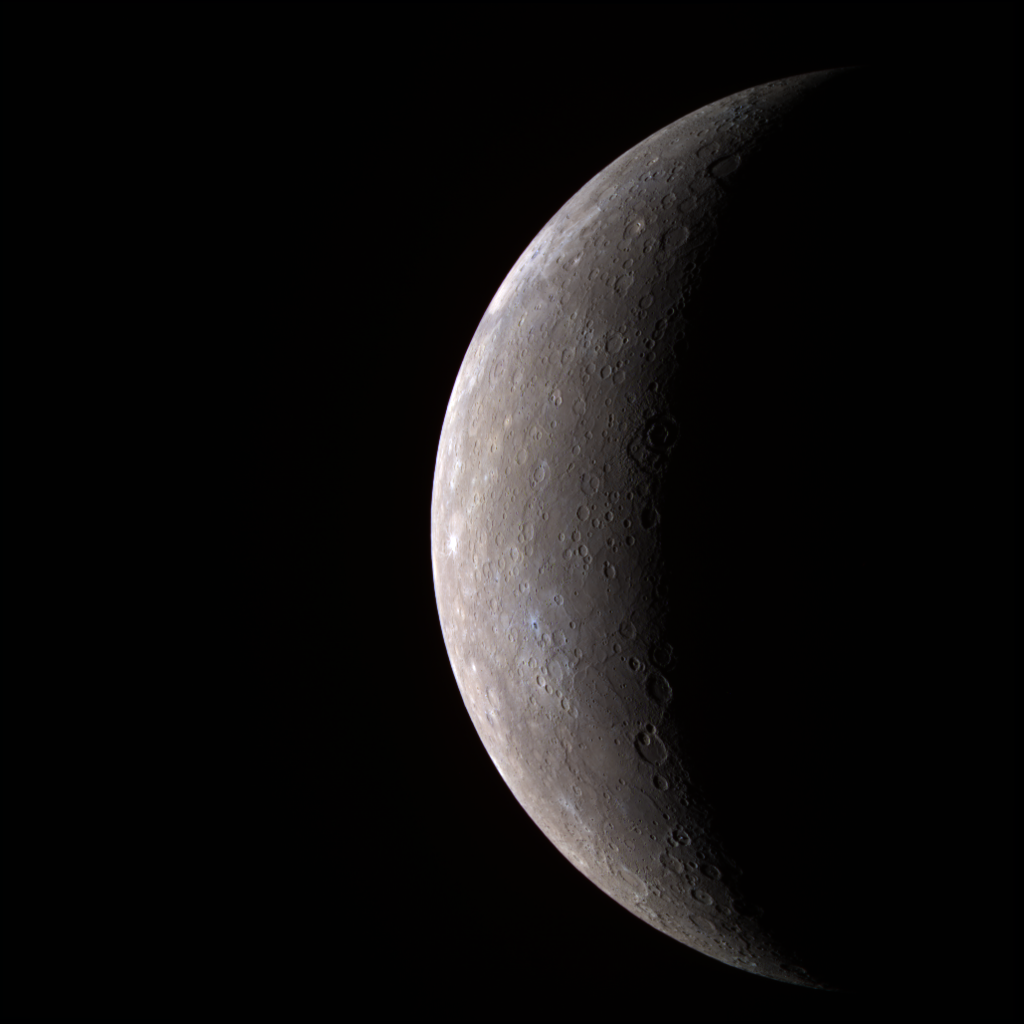
\includegraphics[height=4.65cm]{assets/mercury_messenger.png}};
    \end{tikzpicture}

    \vspace{0.1cm}
    \imgcredit{Mercúrio em cor realçada, NASA/MESSENGER, domínio público}

    \column{0.51\textwidth}
    Mercúrio é pequeno, rápido e muito próximo do Sol.

    \vspace{0.25cm}
    Isso torna a órbita dele um lugar excelente para testar gravitação:
    \begin{itemize}
      \item campo gravitacional solar relativamente forte;
      \item velocidade orbital alta;
      \item muitas voltas acumuladas por século;
      \item órbita excêntrica, com periélio bem definido.
    \end{itemize}

    \vspace{0.15cm}
    A assinatura é pequena, mas sistemática.
  \end{columns}
\end{frame}

\begin{frame}{O que é precessão orbital?}
  \begin{columns}[T,onlytextwidth]
    \column{0.56\textwidth}
    Em uma órbita kepleriana ideal, o periélio permanece fixo.

    \vspace{0.4cm}
    Na prática, a elipse gira lentamente no plano orbital:
    \[
      \Delta\varpi \neq 0.
    \]

    \vspace{0.25cm}
    Para Mercúrio, esse efeito é especialmente visível porque:
    \begin{itemize}
      \item sua órbita é bastante excêntrica;
      \item está muito perto do Sol;
      \item acumula muitas revoluções por século.
    \end{itemize}

    \column{0.4\textwidth}
    \centering
    \begin{tikzpicture}[scale=0.84]
      \coordinate (sun) at (1.18,0);
      \draw[thick,blue!65] (0.35,0) ellipse (1.7 and 0.95);
      \draw[thick,red!70,dashed,rotate=18] (0.35,0) ellipse (1.7 and 0.95);
      \draw[->,thick] (1.95,0) arc[start angle=0,end angle=18,radius=1.95];
      \node at (2.35,0.38) {$\Delta\varpi$};
      \fill[yellow!70!orange] (sun) circle (0.15);
      \node[below] at ([yshift=-0.12cm]sun) {Sol};
      \fill[blue!70] (2.05,0) circle (0.06);
      \fill[red!70] (2.0,0.65) circle (0.06);
      \node[right] at (2.1,0) {periélio};
    \end{tikzpicture}
  \end{columns}
\end{frame}

\begin{frame}{Parâmetros orbitais de Mercúrio}
  \begin{table}
    \centering
    \begin{tabular}{lll}
      \toprule
      Grandeza & Valor aproximado & Por que importa \\
      \midrule
      Semi-eixo maior $a$ & $\SI{0.387}{UA}$ & proximidade do Sol \\
      Excentricidade $e$ & $0{,}206$ & periélio bem marcado \\
      Período orbital & $\SI{87.97}{dias}$ & muitas órbitas/século \\
      Periélio & $\SI{0.307}{UA}$ & campo solar mais forte \\
      Velocidade média & $\SI{47.9}{km/s}$ & regime mais relativístico \\
      \bottomrule
    \end{tabular}
  \end{table}

  \vspace{0.35cm}
  Em termos relativísticos, o parâmetro pequeno é
  \[
    \frac{GM_\odot}{a c^2}\sim 10^{-8}.
  \]
  Pequeno, mas mensurável quando acumulado ao longo de muitas órbitas.
\end{frame}

\begin{frame}{A escala do efeito}
  \centering
  \begin{tikzpicture}[x=0.83cm,y=0.055cm]
    \draw[MercuryLine] (0,0) -- (10,0);
    \foreach \x/\lab in {0/0,2/1000,4/2000,6/3000,8/4000,10/5000} {
      \draw[MercuryLine] (\x,0) -- (\x,-3);
      \node[below,scale=0.7,text=MercuryMuted] at (\x,-3) {\lab};
    }
    \fill[MercuryAccent] (0,12) rectangle (10.05,20);
    \node[right,text=MercuryText,scale=0.82] at (10.2,16) {precessão dos equinócios $\sim 5025\arcsec$};

    \fill[MercuryOrbit] (0,38) rectangle (1.06,46);
    \node[right,text=MercuryText,scale=0.82] at (1.2,42) {perturbações planetárias $\sim 531\arcsec$};

    \fill[MercuryRelativity] (0,64) rectangle (0.086,72);
    \node[right,text=MercuryText,scale=0.82] at (0.22,68) {resíduo relativístico $\sim 43\arcsec$};

    \node[below,text=MercuryMuted,scale=0.8] at (5,-10) {segundos de arco por século};
  \end{tikzpicture}

  \vspace{0.35cm}
  O desafio histórico foi separar uma assinatura pequena dentro de um movimento total muito maior.
\end{frame}

\begin{frame}{O caso de Mercúrio}
  A longitude do periélio de Mercúrio avança cerca de
  \[
    5600\arcsec \text{ por século}
  \]
  quando medida em relação ao equinócio terrestre.

  \vspace{0.35cm}
  A maior parte desse valor não é misteriosa:
  \begin{itemize}
    \item mudança do sistema de referência: precessão dos equinócios;
    \item perturbações gravitacionais dos outros planetas;
    \item pequenos efeitos ligados à forma e ao movimento do Sol.
  \end{itemize}

  \vspace{0.35cm}
  O problema histórico era o resíduo persistente:
  \[
    \Delta\varpi_{\text{anomalia}} \approx 43\arcsec/\text{século}.
  \]
\end{frame}

\section{Contexto histórico}

\begin{frame}{A tradição newtoniana: um enorme sucesso}
  \begin{columns}[T,onlytextwidth]
    \column{0.34\textwidth}
    \centering
    \begin{tikzpicture}
      \node[
        draw=MercuryLine,
        line width=0.45pt,
        inner sep=2pt
      ]{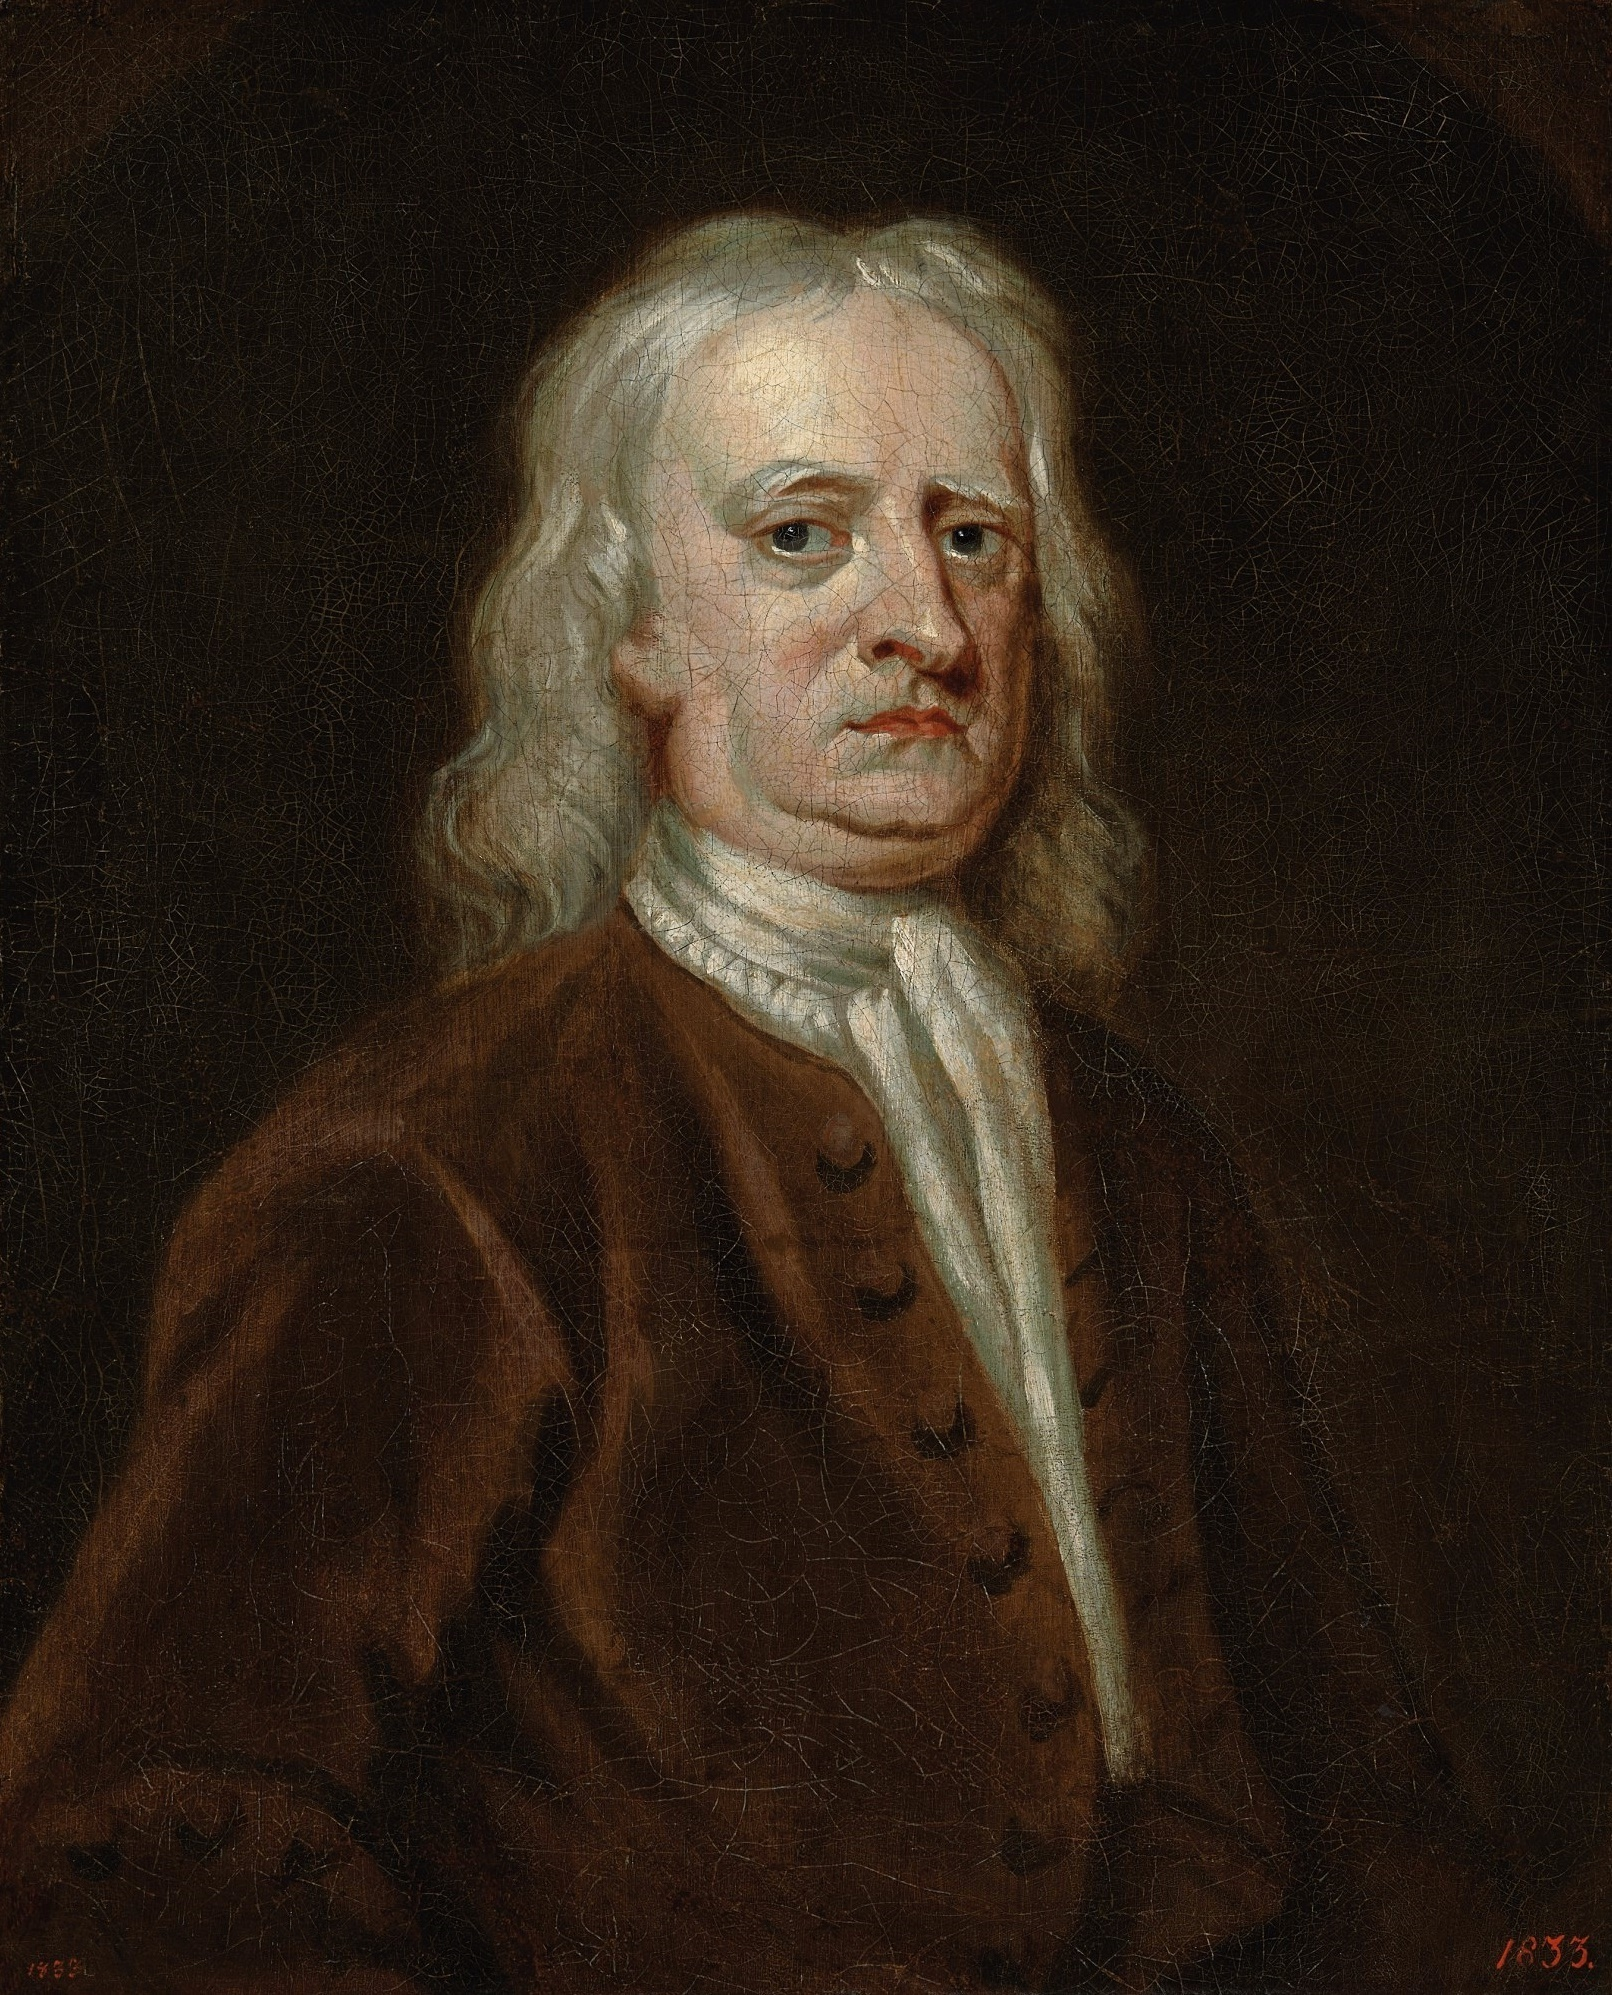
\includegraphics[height=5.05cm]{assets/isaac_newton.jpg}};
    \end{tikzpicture}

    \vspace{0.1cm}
    \imgcredit{Isaac Newton, Wikimedia Commons}

    \column{0.62\textwidth}
    A gravitação universal transformou astronomia em cálculo.

    \vspace{0.25cm}
    \begin{itemize}
      \item A mesma lei explica queda de corpos e órbitas planetárias.
      \item As leis de Kepler aparecem como consequência.
      \item Pequenas diferenças passam a ser interpretadas como perturbações calculáveis.
    \end{itemize}

    \vspace{0.25cm}
    No século XIX, a pergunta não era se Newton funcionava. Era até onde ele funcionava.
  \end{columns}
\end{frame}

\begin{frame}{Linha do tempo do problema}
  \centering
  \begin{tikzpicture}[x=1cm,y=1cm]
    \draw[MercuryLine,line width=0.6pt] (0,0) -- (11,0);
    \foreach \x/\year/\txt in {
      0.5/1687/Newton publica os \textit{Principia},
      3.2/1846/Netuno é previsto e observado,
      5.3/1859/Le Verrier anuncia o resíduo de Mercúrio,
      7.6/1915/Einstein calcula os $43\arcsec$,
      9.4/1919/Eclipse: Sobral e Príncipe,
      10.9/1925/Einstein no Brasil
    } {
      \fill[MercuryAccent] (\x,0) circle (0.055);
      \draw[MercuryLine] (\x,0) -- (\x,0.7);
      \node[above,text=MercuryText,scale=0.76,align=center,text width=2.4cm] at (\x,0.72) {\year\\ \txt};
    }
  \end{tikzpicture}

  \vspace{1.2cm}
  A história de Mercúrio atravessa quase 250 anos: de uma teoria extremamente bem-sucedida a uma nova concepção de espaço e tempo.
\end{frame}

\begin{frame}{Le Verrier e a precisão da mecânica celeste}
  \begin{columns}[T,onlytextwidth]
    \column{0.35\textwidth}
    \centering
    \begin{tikzpicture}
      \node[
        draw=MercuryLine,
        line width=0.45pt,
        inner sep=2pt
      ]{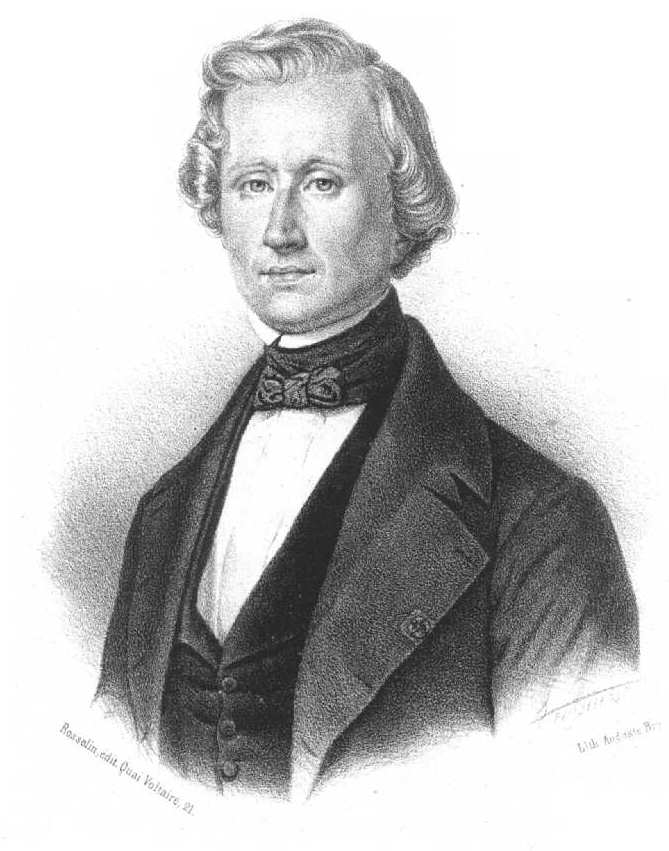
\includegraphics[height=4.85cm]{assets/urbain_le_verrier.jpg}};
    \end{tikzpicture}

    \vspace{0.1cm}
    \imgcredit{Urbain Le Verrier, Wikimedia Commons}

    \column{0.61\textwidth}
    \begin{itemize}
      \item Em 1846, Urbain Le Verrier ficou célebre ao prever Netuno a partir de perturbações na órbita de Urano.
      \item Esse sucesso fortaleceu a confiança no programa newtoniano: discrepâncias orbitais poderiam revelar matéria ainda não observada.
      \item Em 1859, Le Verrier analisou a órbita de Mercúrio e encontrou uma precessão residual do periélio.
    \end{itemize}

    \vspace{0.35cm}
    A pergunta natural era:
    \[
      \text{há uma massa desconhecida perturbando Mercúrio?}
    \]
  \end{columns}
\end{frame}

\begin{frame}{Netuno como precedente metodológico}
  \begin{columns}[T,onlytextwidth]
    \column{0.58\textwidth}
    A descoberta de Netuno criou um roteiro poderoso:

    \vspace{0.18cm}
    \begin{enumerate}
      \item observar uma discrepância orbital;
      \item calcular a perturbação que faltava;
      \item apontar o telescópio para a região prevista;
      \item encontrar um novo corpo celeste.
    \end{enumerate}

    \vspace{0.25cm}
    Para Mercúrio, parecia razoável repetir a estratégia:
    \[
      \text{anomalia orbital} \Longrightarrow \text{planeta intramercurial?}
    \]

    \vspace{0.18cm}
    A força da hipótese de Vulcano vinha menos da fantasia e mais do sucesso anterior da mecânica celeste.

    \column{0.36\textwidth}
    \centering
    \begin{tikzpicture}
      \node[
        draw=MercuryLine,
        line width=0.45pt,
        inner sep=2pt
      ]{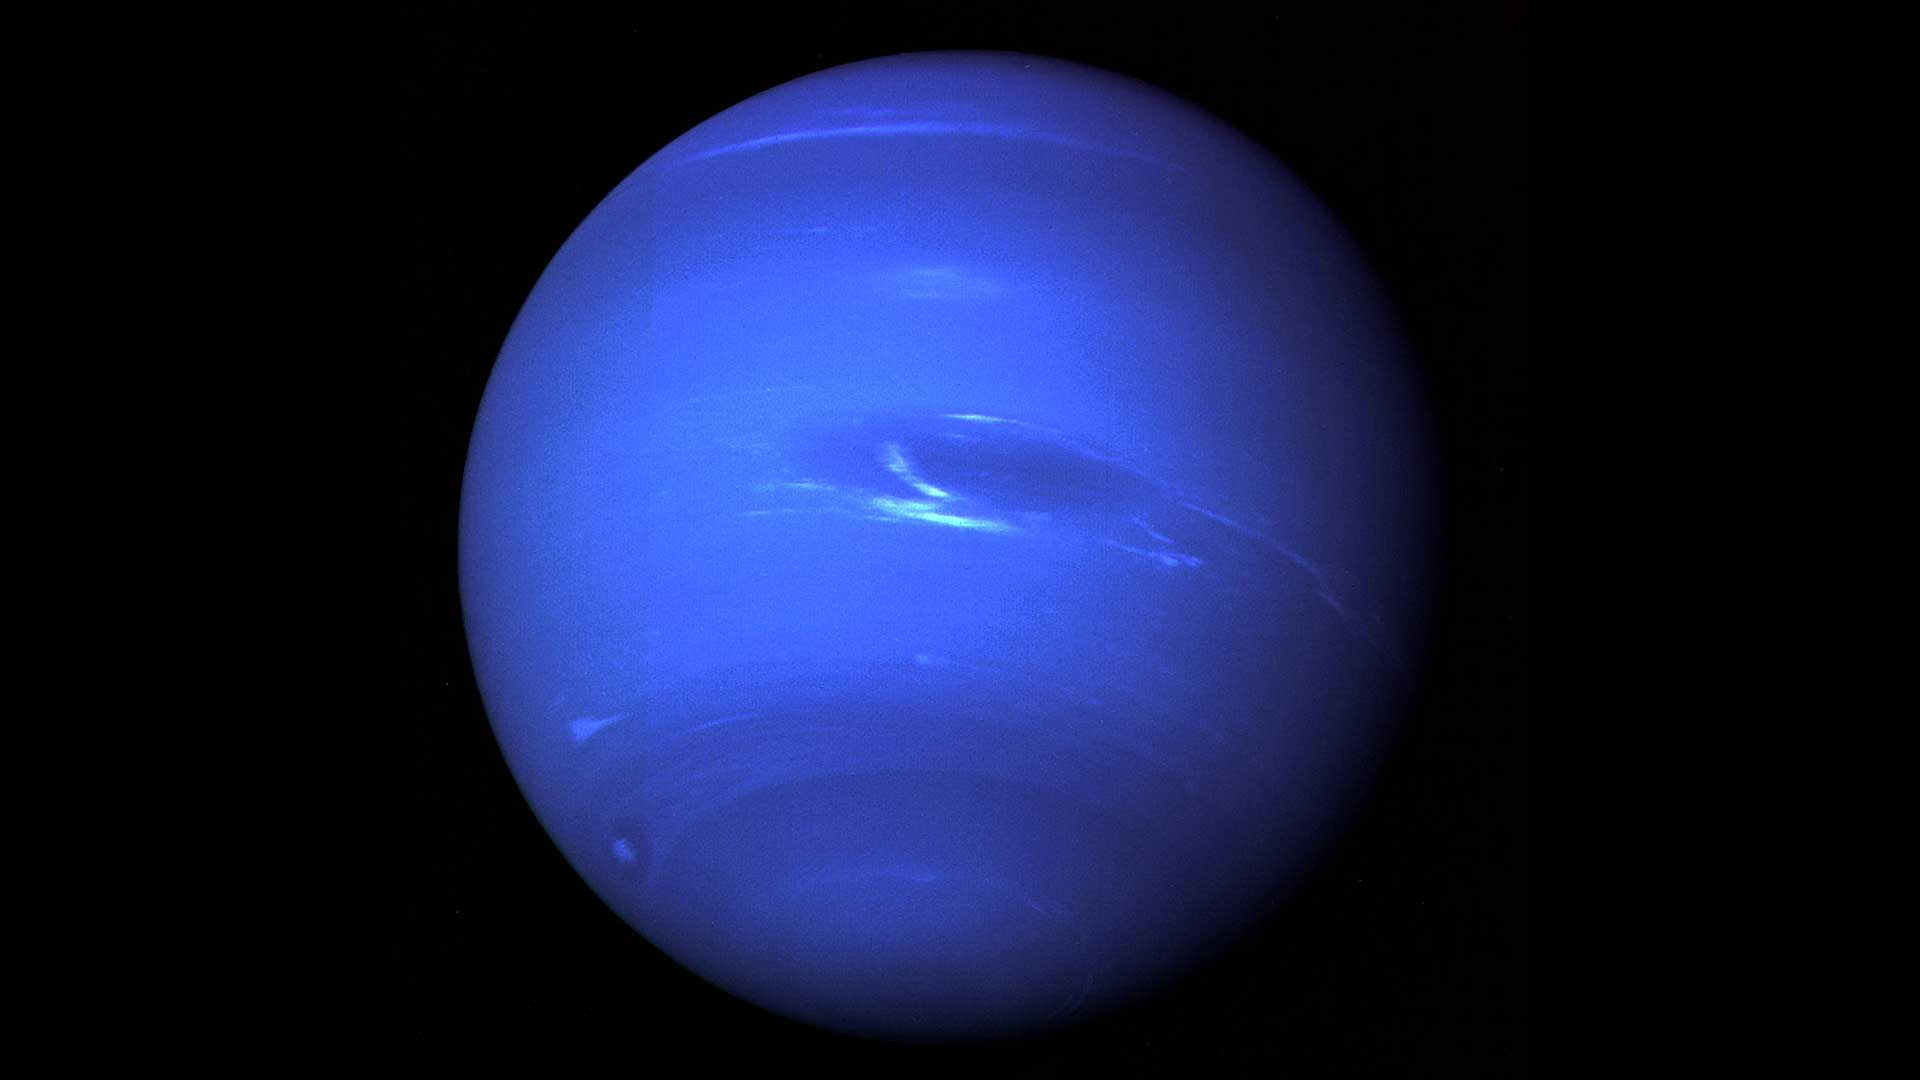
\includegraphics[width=0.95\linewidth]{assets/neptune_voyager2.jpg}};
    \end{tikzpicture}

    \vspace{0.08cm}
    \imgcredit{Voyager 2, NASA/JPL-Caltech}
  \end{columns}
\end{frame}

\begin{frame}{A hipótese de Vulcano}
  \begin{columns}[T,onlytextwidth]
    \column{0.58\textwidth}
    Para explicar o resíduo, foi proposta a existência de um planeta intramercurial:
    \[
      \text{Vulcano, orbitando entre Mercúrio e o Sol.}
    \]

    \vspace{0.25cm}
    A hipótese era plausível dentro da física da época:
    \begin{itemize}
      \item repetia a lógica bem-sucedida da descoberta de Netuno;
      \item introduzia uma fonte newtoniana adicional;
      \item poderia produzir uma precessão extra.
    \end{itemize}

    \vspace{0.25cm}
    Mas as supostas observações de Vulcano nunca se tornaram reprodutíveis.

    \column{0.36\textwidth}
    \centering
    \begin{tikzpicture}
      \node[
        draw=MercuryLine,
        line width=0.45pt,
        inner sep=2.5pt
      ] {
        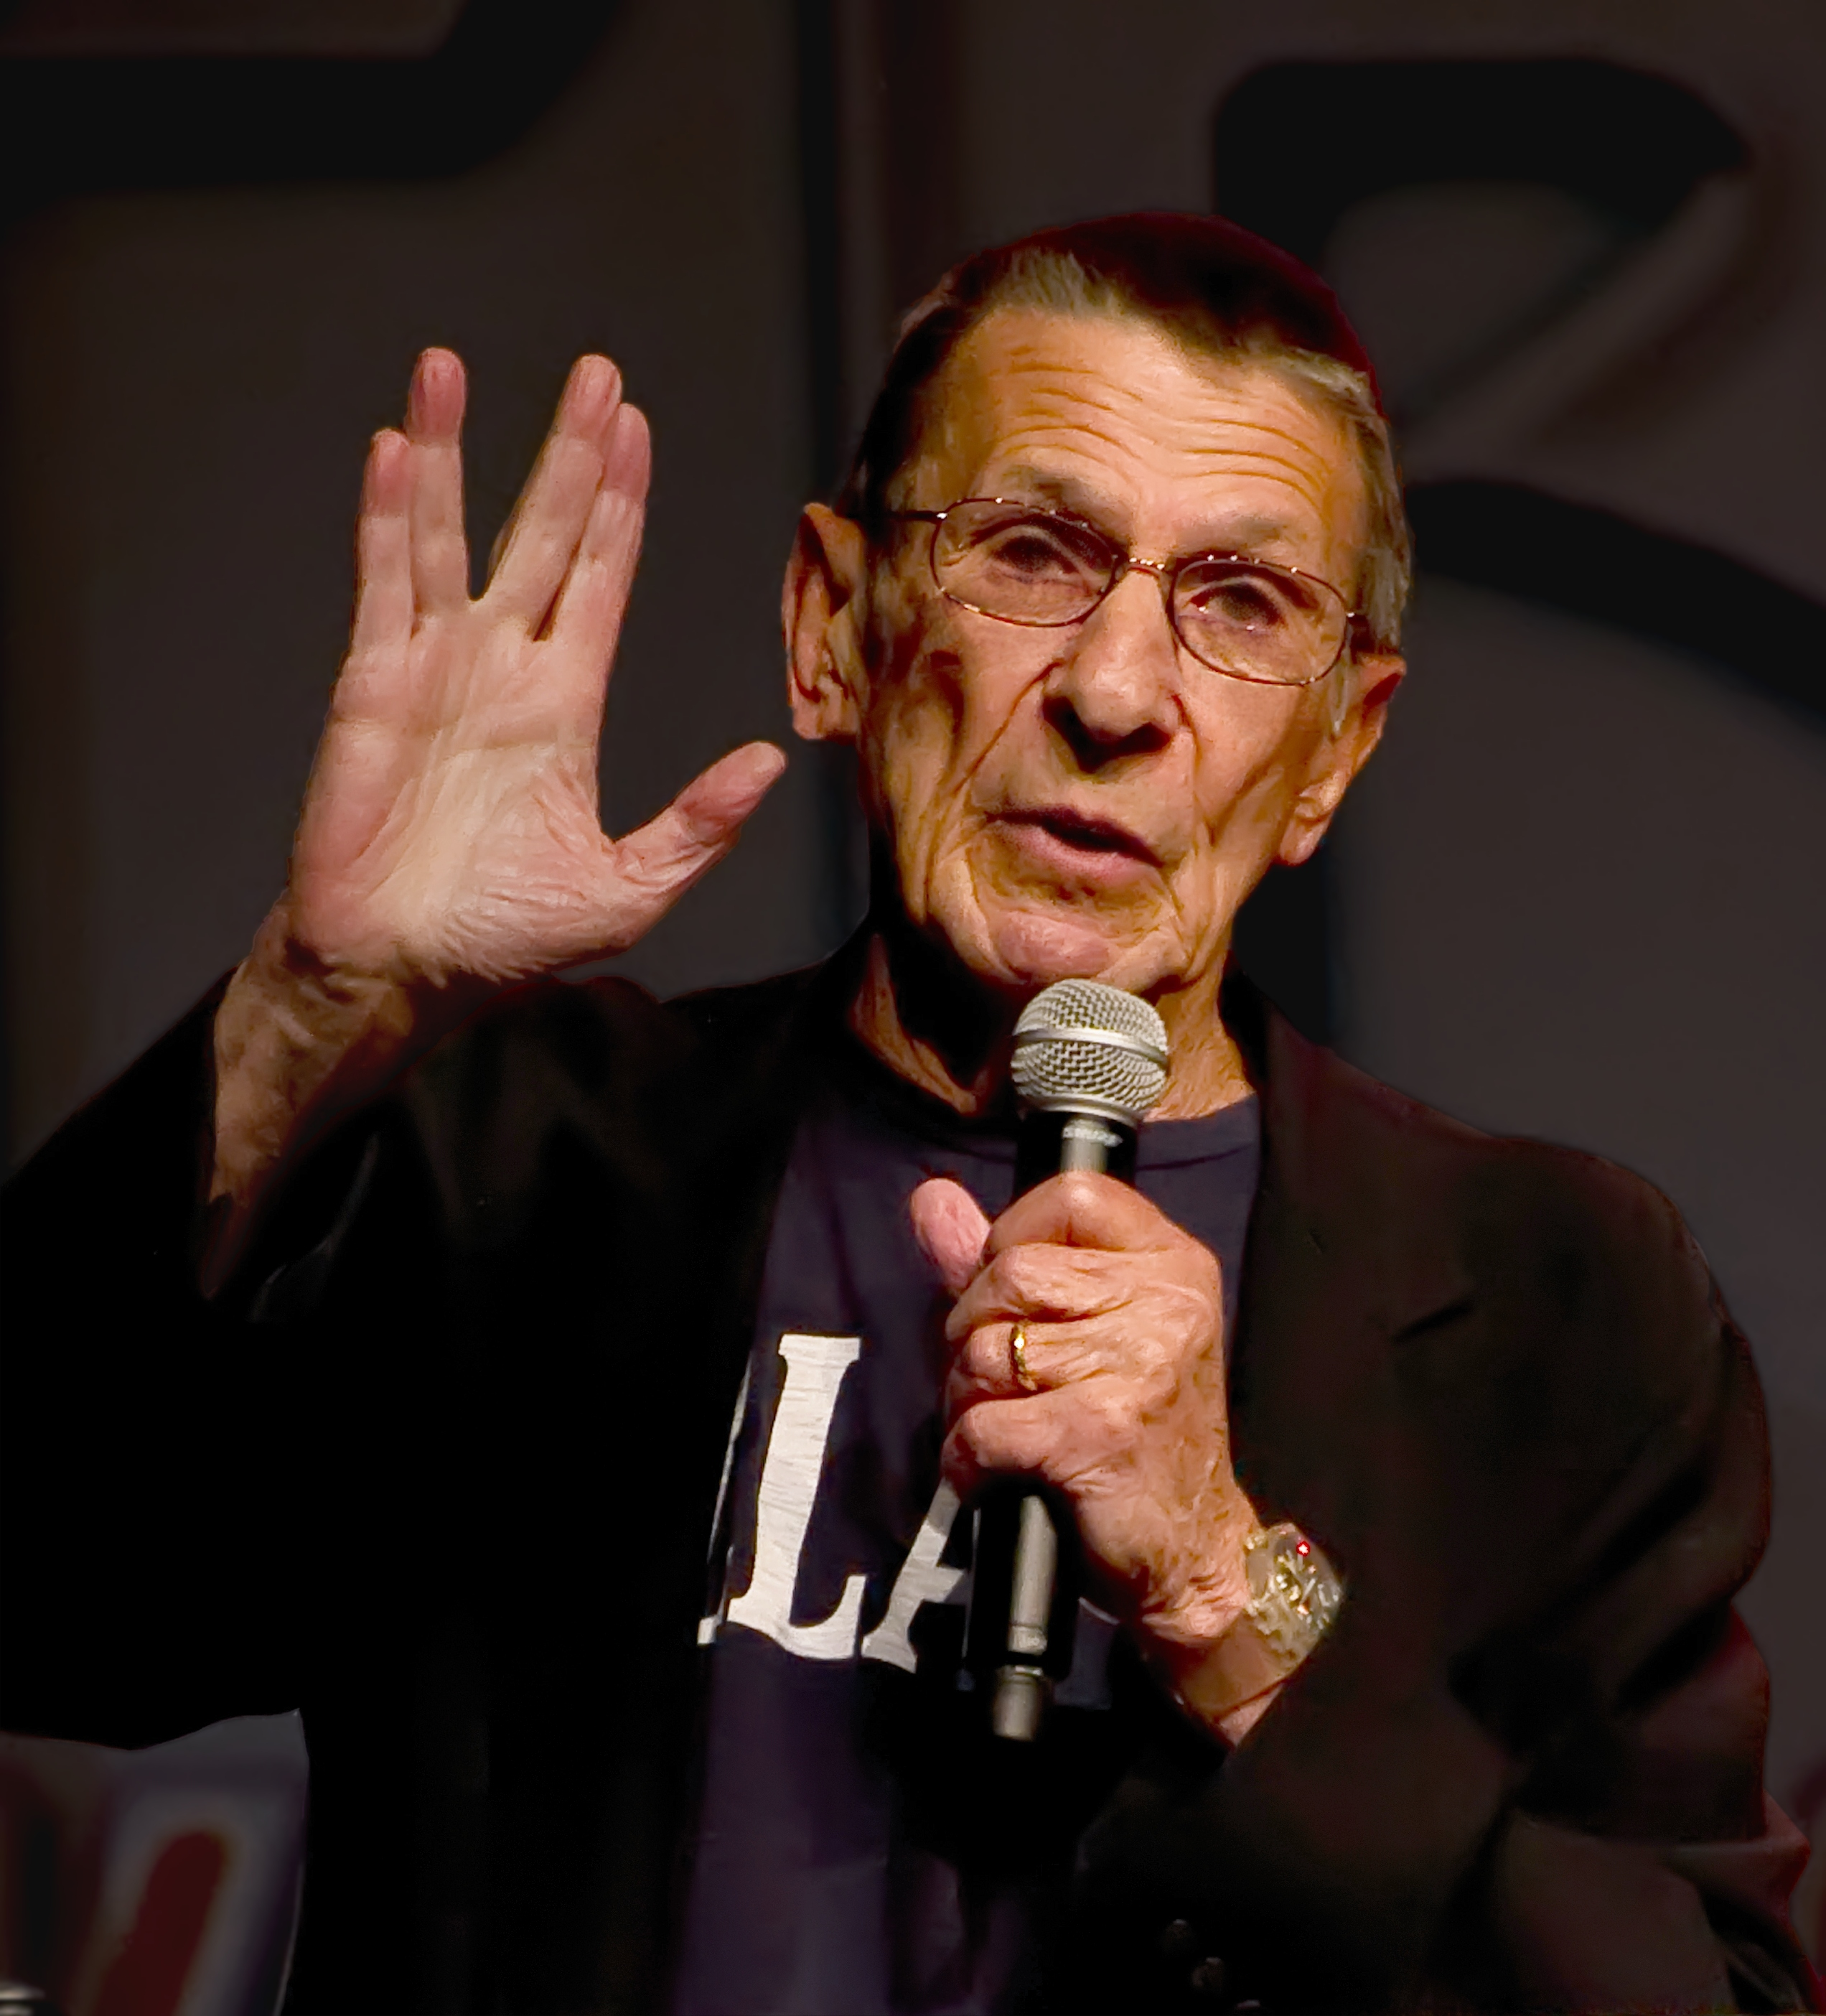
\includegraphics[height=4.45cm]{assets/leonard_nimoy_vulcan_salute.jpg}
      };
    \end{tikzpicture}

    \vspace{0.1cm}
    {\tiny\color{MercuryMuted}
    Leonard Nimoy, CC BY 2.0, Wikimedia Commons}
  \end{columns}
\end{frame}

\section{A inadequação newtoniana}

\begin{frame}{Kepler contra pequenas correções}
  A órbita kepleriana é fechada porque a força é exatamente proporcional a $1/r^2$.

  \vspace{0.25cm}
  Com $u=1/r$, a equação orbital newtoniana ideal tem a forma
  \[
    \frac{d^2u}{d\phi^2}+u=\frac{GM}{h^2}.
  \]

  \vspace{0.25cm}
  A solução é periódica em $\phi$:
  \[
    u(\phi)=\frac{GM}{h^2}\left(1+e\cos\phi\right).
  \]

  \vspace{0.3cm}
  Qualquer termo extra pequeno pode quebrar esse fechamento perfeito.
\end{frame}

\begin{frame}{O que Newton prevê?}
  Para uma força central exatamente inversa ao quadrado,
  \[
    F(r) = -\frac{GMm}{r^2},
  \]
  as órbitas ligadas são elipses fechadas:
  \[
    r(\phi)=\frac{a(1-e^2)}{1+e\cos\phi}.
  \]

  \vspace{0.35cm}
  Isso significa que, no problema de dois corpos isolado:
  \[
    \Delta\varpi_{\text{Newton, 2 corpos}} = 0.
  \]

  \vspace{0.35cm}
  Portanto, a precessão observada só poderia vir de perturbações: planetas, achatamento solar, poeira, massas não vistas ou correções à lei gravitacional.
\end{frame}

\begin{frame}{O resíduo em gráfico}
  \centering
  \begin{tikzpicture}[x=0.08cm,y=0.8cm]
    \draw[MercuryLine] (0,0) -- (75,0);
    \foreach \x/\lab in {0/0,15/150,30/300,45/450,60/600,75/750} {
      \draw[MercuryLine] (\x,0) -- (\x,-0.08);
      \node[below,text=MercuryMuted,scale=0.7] at (\x,-0.1) {\lab};
    }
    \fill[MercuryOrbit] (0,1.2) rectangle (53.1,1.65);
    \node[left,text=MercuryText,scale=0.83] at (-1,1.425) {planetas};
    \node[right,text=MercuryText,scale=0.83] at (54.2,1.425) {$531\arcsec$};

    \fill[MercuryRelativity] (0,2.15) rectangle (4.3,2.6);
    \node[left,text=MercuryText,scale=0.83] at (-1,2.375) {anomalia};
    \node[right,text=MercuryText,scale=0.83] at (5.4,2.375) {$43\arcsec$};

    \fill[MercuryAccent] (0,3.1) rectangle (1.0,3.55);
    \node[left,text=MercuryText,scale=0.83] at (-1,3.325) {efeitos menores};
    \node[right,text=MercuryText,scale=0.83] at (2.1,3.325) {pequenos};

    \node[below,text=MercuryMuted,scale=0.78] at (37,-0.55) {segundos de arco por século, sem a precessão dos equinócios};
  \end{tikzpicture}

  \vspace{0.4cm}
  Depois de remover os efeitos conhecidos, o que sobra é pequeno, mas não desaparece.
\end{frame}

\begin{frame}{Perturbações planetárias: quase tudo, mas não tudo}
  \begin{table}
    \centering
    \begin{tabular}{ll}
      \toprule
      Contribuição & {Avanço do periélio $(\arcsec/\text{século})$} \\
      \midrule
      Precessão dos equinócios & 5025 \\
      Perturbações dos planetas & 531 \\
      Achatamento solar e efeitos menores & pequeno \\
      \midrule
      Resíduo histórico & 43 \\
      \bottomrule
    \end{tabular}
  \end{table}

  \vspace{0.25cm}
  O ponto crucial não era que Newton ``falhava muito'', mas que falhava pouco e de modo sistemático.

  \vspace{0.2cm}
  Essa pequena diferença estava acima dos erros observacionais acumulados.
\end{frame}

\begin{frame}{Tentativas newtonianas de solução}
  Antes de Einstein, foram consideradas várias saídas:

  \begin{itemize}
    \item um planeta intramercurial, Vulcano;
    \item um anel de pequenos corpos perto do Sol;
    \item mudanças empíricas na lei de força;
    \item efeitos do achatamento do Sol.
  \end{itemize}

  \vspace{0.35cm}
  O problema é que essas hipóteses exigiam evidências independentes ou geravam conflitos com outras órbitas planetárias.

  \vspace{0.35cm}
  A anomalia de Mercúrio virou um teste sensível para qualquer teoria gravitacional mais profunda.
\end{frame}

\section{A solução relativística}

\begin{frame}{Aula 2 começa aqui: a gravidade muda de papel}
  \centering
  \vspace{0.6cm}
  {\Large\color{MercuryText}De uma força entre massas}

  \vspace{0.25cm}
  {\color{MercuryAccent}\Large$\Downarrow$}

  \vspace{0.25cm}
  {\Large\color{MercuryText}para a geometria do espaço-tempo}

  \vspace{0.7cm}
  \begin{tikzpicture}[scale=0.85]
    \draw[MercuryLine] (-4,-1) grid[step=0.5] (4,1);
    \foreach \x in {-4,-3.5,...,4} {
      \draw[MercuryLine] (\x,-1) .. controls (\x*0.75,-0.2) and (\x*0.75,0.2) .. (\x,1);
    }
    \fill[MercuryAccent] (0,0) circle (0.16);
    \node[below,text=MercuryMuted] at (0,-1.25) {massa curva a geometria; trajetórias livres seguem essa geometria};
  \end{tikzpicture}
\end{frame}

\begin{frame}{A ideia central da relatividade geral}
  Na relatividade geral, a gravidade não é uma força no sentido newtoniano.

  \vspace{0.25cm}
  A presença de massa e energia curva o espaço-tempo, e os corpos livres seguem geodésicas:
  \[
    G_{\mu\nu} = \frac{8\pi G}{c^4}T_{\mu\nu}.
  \]

  \vspace{0.35cm}
  Para uma partícula orbitando o Sol, a geometria relevante, em primeira aproximação, é a métrica de Schwarzschild:
  \[
    ds^2 =
    -\left(1-\frac{2GM}{c^2r}\right)c^2dt^2
    +\left(1-\frac{2GM}{c^2r}\right)^{-1}dr^2
    +r^2d\Omega^2.
  \]
\end{frame}

\begin{frame}{Quanto a precessão depende da órbita?}
  \centering
  \begin{tikzpicture}[x=3.25cm,y=3.55cm]
    \draw[MercuryLine] (0,0) rectangle (2.5,1.15);
    \foreach \i/\a in {0/0.3,1/0.6,2/1.0,3/1.5,4/2.0} {
      \draw[MercuryLine] ({\i*0.625},0) -- ({\i*0.625},-0.025);
      \node[below,text=MercuryMuted,scale=0.65] at ({\i*0.625},-0.035) {\a};
    }
    \foreach \j/\e in {0/0,1/0.2,2/0.4,3/0.6,4/0.8} {
      \draw[MercuryLine] (0,{\j*0.2875}) -- (-0.025,{\j*0.2875});
      \node[left,text=MercuryMuted,scale=0.65] at (-0.035,{\j*0.2875}) {\e};
    }
    \foreach \x/\y/\c in {
      0.15/0.10/90,0.45/0.10/80,0.75/0.10/70,1.05/0.10/55,1.35/0.10/40,1.65/0.10/25,2.05/0.10/15,
      0.15/0.40/95,0.45/0.40/84,0.75/0.40/72,1.05/0.40/58,1.35/0.40/43,1.65/0.40/30,2.05/0.40/18,
      0.15/0.70/100,0.45/0.70/90,0.75/0.70/80,1.05/0.70/65,1.35/0.70/50,1.65/0.70/35,2.05/0.70/22,
      0.15/1.00/100,0.45/1.00/96,0.75/1.00/88,1.05/1.00/75,1.35/1.00/62,1.65/1.00/48,2.05/1.00/35
    } {
      \fill[MercuryRelativity!\c!MercuryBlack] (\x,\y) rectangle +(0.25,0.18);
    }
    \node[below,text=MercuryMuted,scale=0.8] at (1.25,-0.16) {$a$ em UA};
    \node[rotate=90,text=MercuryMuted,scale=0.8] at (-0.32,0.58) {$e$};
  \end{tikzpicture}

  \vspace{0.18cm}
  Quanto menor $a$ e maior $e$, maior é $\Delta\varpi$.
  Mercúrio está no canto favorável do Sistema Solar.
\end{frame}

\begin{frame}{A correção relativística à órbita}
  Escrevendo $u=1/r$, a equação orbital relativística pode ser aproximada por
  \[
    \frac{d^2u}{d\phi^2}+u
    =
    \frac{GM}{h^2}
    +
    \frac{3GM}{c^2}u^2.
  \]

  \vspace{0.35cm}
  O termo novo,
  \[
    \frac{3GM}{c^2}u^2,
  \]
  não existe na teoria newtoniana.

  \vspace{0.35cm}
  Ele faz a órbita deixar de ser uma elipse perfeitamente fechada: o periélio avança a cada revolução.
\end{frame}

\begin{frame}{Fórmula do avanço do periélio}
  A relatividade geral prevê, por revolução,
  \[
    \Delta\varpi
    =
    \frac{6\pi GM}{a(1-e^2)c^2}.
  \]

  \vspace{0.3cm}
  Para Mercúrio:
  \begin{align*}
    a &\approx \SI{5.79e10}{m}, \\
    e &\approx 0{,}206, \\
    T &\approx \SI{87.97}{dias}.
  \end{align*}

  \vspace{0.25cm}
  Convertendo para segundos de arco por século:
  \[
    \Delta\varpi_{\text{RG}}
    \approx 43\arcsec/\text{século}.
  \]
\end{frame}

\begin{frame}{Por que Mercúrio é o melhor teste?}
  A correção relativística escala como
  \[
    \Delta\varpi \propto \frac{1}{a(1-e^2)}.
  \]

  \vspace{0.3cm}
  Logo, o efeito cresce quando:
  \begin{itemize}
    \item a órbita é pequena, isto é, próxima do Sol;
    \item a excentricidade é maior;
    \item o corpo completa muitas órbitas em pouco tempo.
  \end{itemize}

  \vspace{0.35cm}
  Mercúrio combina exatamente esses fatores. Para planetas mais externos, a precessão relativística existe, mas é menor.

  \vspace{0.3cm}
  {\color{MercuryAccent}
  \href{dashboard_orbita_mercurio.html}{Abrir dashboard interativo: variar $a$ e $e$}}

  \vspace{0.12cm}
  {\tiny\color{MercuryMuted}
  fallback: abrir \texttt{dashboard\_orbita\_mercurio.html} na pasta da apresentação}
\end{frame}

\section{Significado físico}

\begin{frame}{O triunfo de 1915}
  Em novembro de 1915, Einstein aplicou sua nova teoria ao periélio de Mercúrio.

  \vspace{0.35cm}
  O resultado reproduziu justamente o resíduo anômalo:
  \[
    43\arcsec/\text{século}.
  \]

  \vspace{0.35cm}
  Isso foi decisivo porque:
  \begin{itemize}
    \item não exigia Vulcano nem massas invisíveis;
    \item surgia de princípios geométricos gerais;
    \item explicava uma anomalia já conhecida, não apenas uma previsão ajustada depois.
  \end{itemize}
\end{frame}

\begin{frame}{Comparação conceitual}
  \begin{table}
    \centering
    \begin{tabular}{lll}
      \toprule
      Aspecto & Newton & Relatividade geral \\
      \midrule
      Gravidade & força & geometria do espaço-tempo \\
      Espaço e tempo & absolutos & dinâmicos \\
      Órbita ideal & elipse fechada & quase-elipse precessante \\
      Anomalia de Mercúrio & resíduo inexplicado & consequência natural \\
      \bottomrule
    \end{tabular}
  \end{table}

  \vspace{0.35cm}
  A relatividade geral contém a gravitação newtoniana como limite:
  \[
    v \ll c
    \quad\text{e}\quad
    \frac{GM}{rc^2}\ll 1.
  \]
\end{frame}

\section{Sobral, 1919: luz, eclipse e Brasil}

\begin{frame}{Outro teste: a luz também deve curvar}
  Se gravidade é geometria, a luz também segue a geometria do espaço-tempo.

  \vspace{0.3cm}
  Para um raio de luz passando rasante ao Sol, a relatividade geral prevê:
  \[
    \alpha_{\text{RG}} =
    \frac{4GM_\odot}{c^2R_\odot}
    \approx 1{,}75\arcsec.
  \]

  \vspace{0.25cm}
  A previsão newtoniana aproximada para uma partícula de luz seria metade:
  \[
    \alpha_{\text{Newton}} \approx 0{,}87\arcsec.
  \]

  \vspace{0.3cm}
  Medir essa diferença exigia observar estrelas muito próximas do disco solar.
\end{frame}

\begin{frame}{Por que um eclipse total?}
  \begin{columns}[T,onlytextwidth]
    \column{0.55\textwidth}
    Normalmente, o brilho do Sol impede observar estrelas próximas no céu.

    \vspace{0.25cm}
    Durante um eclipse total:
    \begin{itemize}
      \item a Lua bloqueia o disco solar;
      \item estrelas próximas ao Sol tornam-se visíveis;
      \item compara-se a posição aparente das estrelas com placas de referência.
    \end{itemize}

    \vspace{0.25cm}
    O deslocamento esperado era minúsculo, da ordem de segundos de arco.

    \column{0.4\textwidth}
    \centering
    \begin{tikzpicture}[scale=0.95]
      \fill[MercuryAccent] (0,0) circle (0.42);
      \fill[MercuryBlack] (0,0) circle (0.31);
      \draw[MercuryLine] (0,0) circle (0.42);
      \foreach \x/\y in {-1.6/1.1,-1.1/-0.7,1.4/0.9,1.6/-1.0,0.7/1.45,-1.7/0.1} {
        \fill[MercuryText] (\x,\y) circle (0.025);
      }
      \draw[MercuryRelativity,->,line width=0.8pt] (-1.65,1.1) .. controls (-0.6,0.65) and (0.7,0.48) .. (1.7,0.85);
      \node[text=MercuryMuted,scale=0.72] at (0,-1.55) {o eclipse revela estrelas perto do Sol};
    \end{tikzpicture}
  \end{columns}
\end{frame}

\begin{frame}{As expedições de 1919}
  \begin{columns}[T,onlytextwidth]
    \column{0.46\textwidth}
    Duas equipes observaram o eclipse total de \textbf{29 de maio de 1919}:
    \begin{itemize}
      \item Eddington e Cottingham em Príncipe, na costa oeste da África;
      \item Crommelin e Davidson em Sobral, no Ceará;
      \item organização ligada à Royal Society e à Royal Astronomical Society.
    \end{itemize}

    \vspace{0.25cm}
    Einstein não estava em Sobral. Ele estava na Europa, aguardando os resultados.

    \column{0.5\textwidth}
    \centering
    \begin{tikzpicture}[x=1cm,y=1cm]
      \draw[MercuryLine] (-0.5,-1.2) rectangle (5.4,3.2);
      \node[text=MercuryMuted,scale=0.75] at (0.25,2.75) {Europa};
      \node[text=MercuryMuted,scale=0.75] at (2.2,0.5) {Atlântico};
      \node[text=MercuryMuted,scale=0.75] at (4.55,-0.75) {Brasil};
      \node[text=MercuryMuted,scale=0.75] at (2.7,-0.35) {África};

      \fill[MercuryAccent] (0.7,2.2) circle (0.06);
      \node[above,text=MercuryText,scale=0.7] at (0.7,2.25) {Londres};
      \fill[MercuryRelativity] (2.8,0.0) circle (0.06);
      \node[right,text=MercuryText,scale=0.7] at (2.85,0.0) {Príncipe};
      \fill[MercuryOrbit] (4.55,-0.35) circle (0.06);
      \node[right,text=MercuryText,scale=0.7] at (4.6,-0.35) {Sobral};

      \draw[MercuryRelativity,->,line width=0.8pt] (0.7,2.15) .. controls (1.3,1.1) and (2.0,0.4) .. (2.75,0.03);
      \draw[MercuryOrbit,->,line width=0.8pt] (0.75,2.1) .. controls (1.9,0.8) and (3.4,0.1) .. (4.5,-0.32);
    \end{tikzpicture}
  \end{columns}
\end{frame}

\begin{frame}{Sobral nas placas fotográficas}
  \begin{columns}[T,onlytextwidth]
    \column{0.42\textwidth}
    \centering
    \begin{tikzpicture}
      \node[
        draw=MercuryLine,
        line width=0.45pt,
        inner sep=2pt
      ]{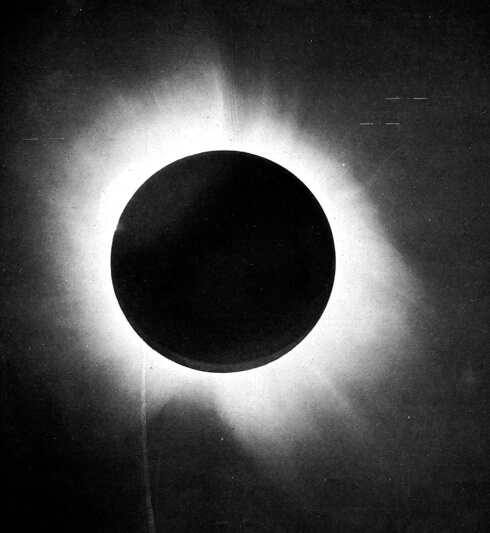
\includegraphics[height=4.65cm]{assets/sobral_1919_eclipse_positive.jpg}};
    \end{tikzpicture}

    \vspace{0.1cm}
    \imgcredit{Placa positiva do eclipse de Sobral, 29/05/1919, domínio público}

    \column{0.54\textwidth}
    O método era fotográfico:
    \begin{itemize}
      \item fotografar estrelas próximas ao Sol durante o eclipse;
      \item fotografar o mesmo campo estelar sem o Sol;
      \item medir deslocamentos em placas de vidro;
      \item inferir a deflexão da luz.
    \end{itemize}

    \vspace{0.25cm}
    O Brasil entrou na história da relatividade porque Sobral estava na faixa de totalidade e teve condições observacionais decisivas.
  \end{columns}
\end{frame}

\begin{frame}{Resultados: perto de Einstein}
  \begin{table}
    \centering
    \begin{tabular}{lll}
      \toprule
      Conjunto de dados & Deflexão medida & Interpretação histórica \\
      \midrule
      Sobral, lente de 4 pol. & $1{,}98\arcsec \pm 0{,}16\arcsec$ & próximo de Einstein \\
      Príncipe & $1{,}61\arcsec \pm 0{,}40\arcsec$ & compatível com Einstein \\
      Sobral, astrográfico & $\sim 0{,}93\arcsec$ & descartado por problemas ópticos \\
      \bottomrule
    \end{tabular}
  \end{table}

  \vspace{0.35cm}
  Em 6 de novembro de 1919, os resultados foram anunciados em Londres.

  \vspace{0.25cm}
  A partir daí, Einstein deixou de ser apenas conhecido entre físicos e virou figura pública mundial.
\end{frame}

\begin{frame}{Mito e história: Einstein veio a Sobral?}
  \begin{columns}[T,onlytextwidth]
    \column{0.5\textwidth}
    {\color{MercuryAccent}\textbf{Não.}}

    \vspace{0.2cm}
    O eclipse de Sobral aconteceu em \textbf{29 de maio de 1919}.

    \vspace{0.2cm}
    As equipes estrangeiras em campo foram:
    \begin{itemize}
      \item Crommelin e Davidson em Sobral;
      \item Eddington e Cottingham em Príncipe.
    \end{itemize}

    \vspace{0.2cm}
    Einstein não participou da viagem observacional.

    \column{0.46\textwidth}
    {\color{MercuryAccent}\textbf{Sim, Einstein veio ao Brasil depois.}}

    \vspace{0.2cm}
    Ele visitou o Rio de Janeiro entre \textbf{4 e 12 de maio de 1925}.

    \vspace{0.2cm}
    O eclipse de Sobral já havia tornado a relatividade geral famosa seis anos antes.
  \end{columns}
\end{frame}

\begin{frame}{Einstein no Brasil, 1925}
  \begin{columns}[T,onlytextwidth]
    \column{0.52\textwidth}
    \centering
    \begin{tikzpicture}
      \node[
        draw=MercuryLine,
        line width=0.45pt,
        inner sep=2pt
      ]{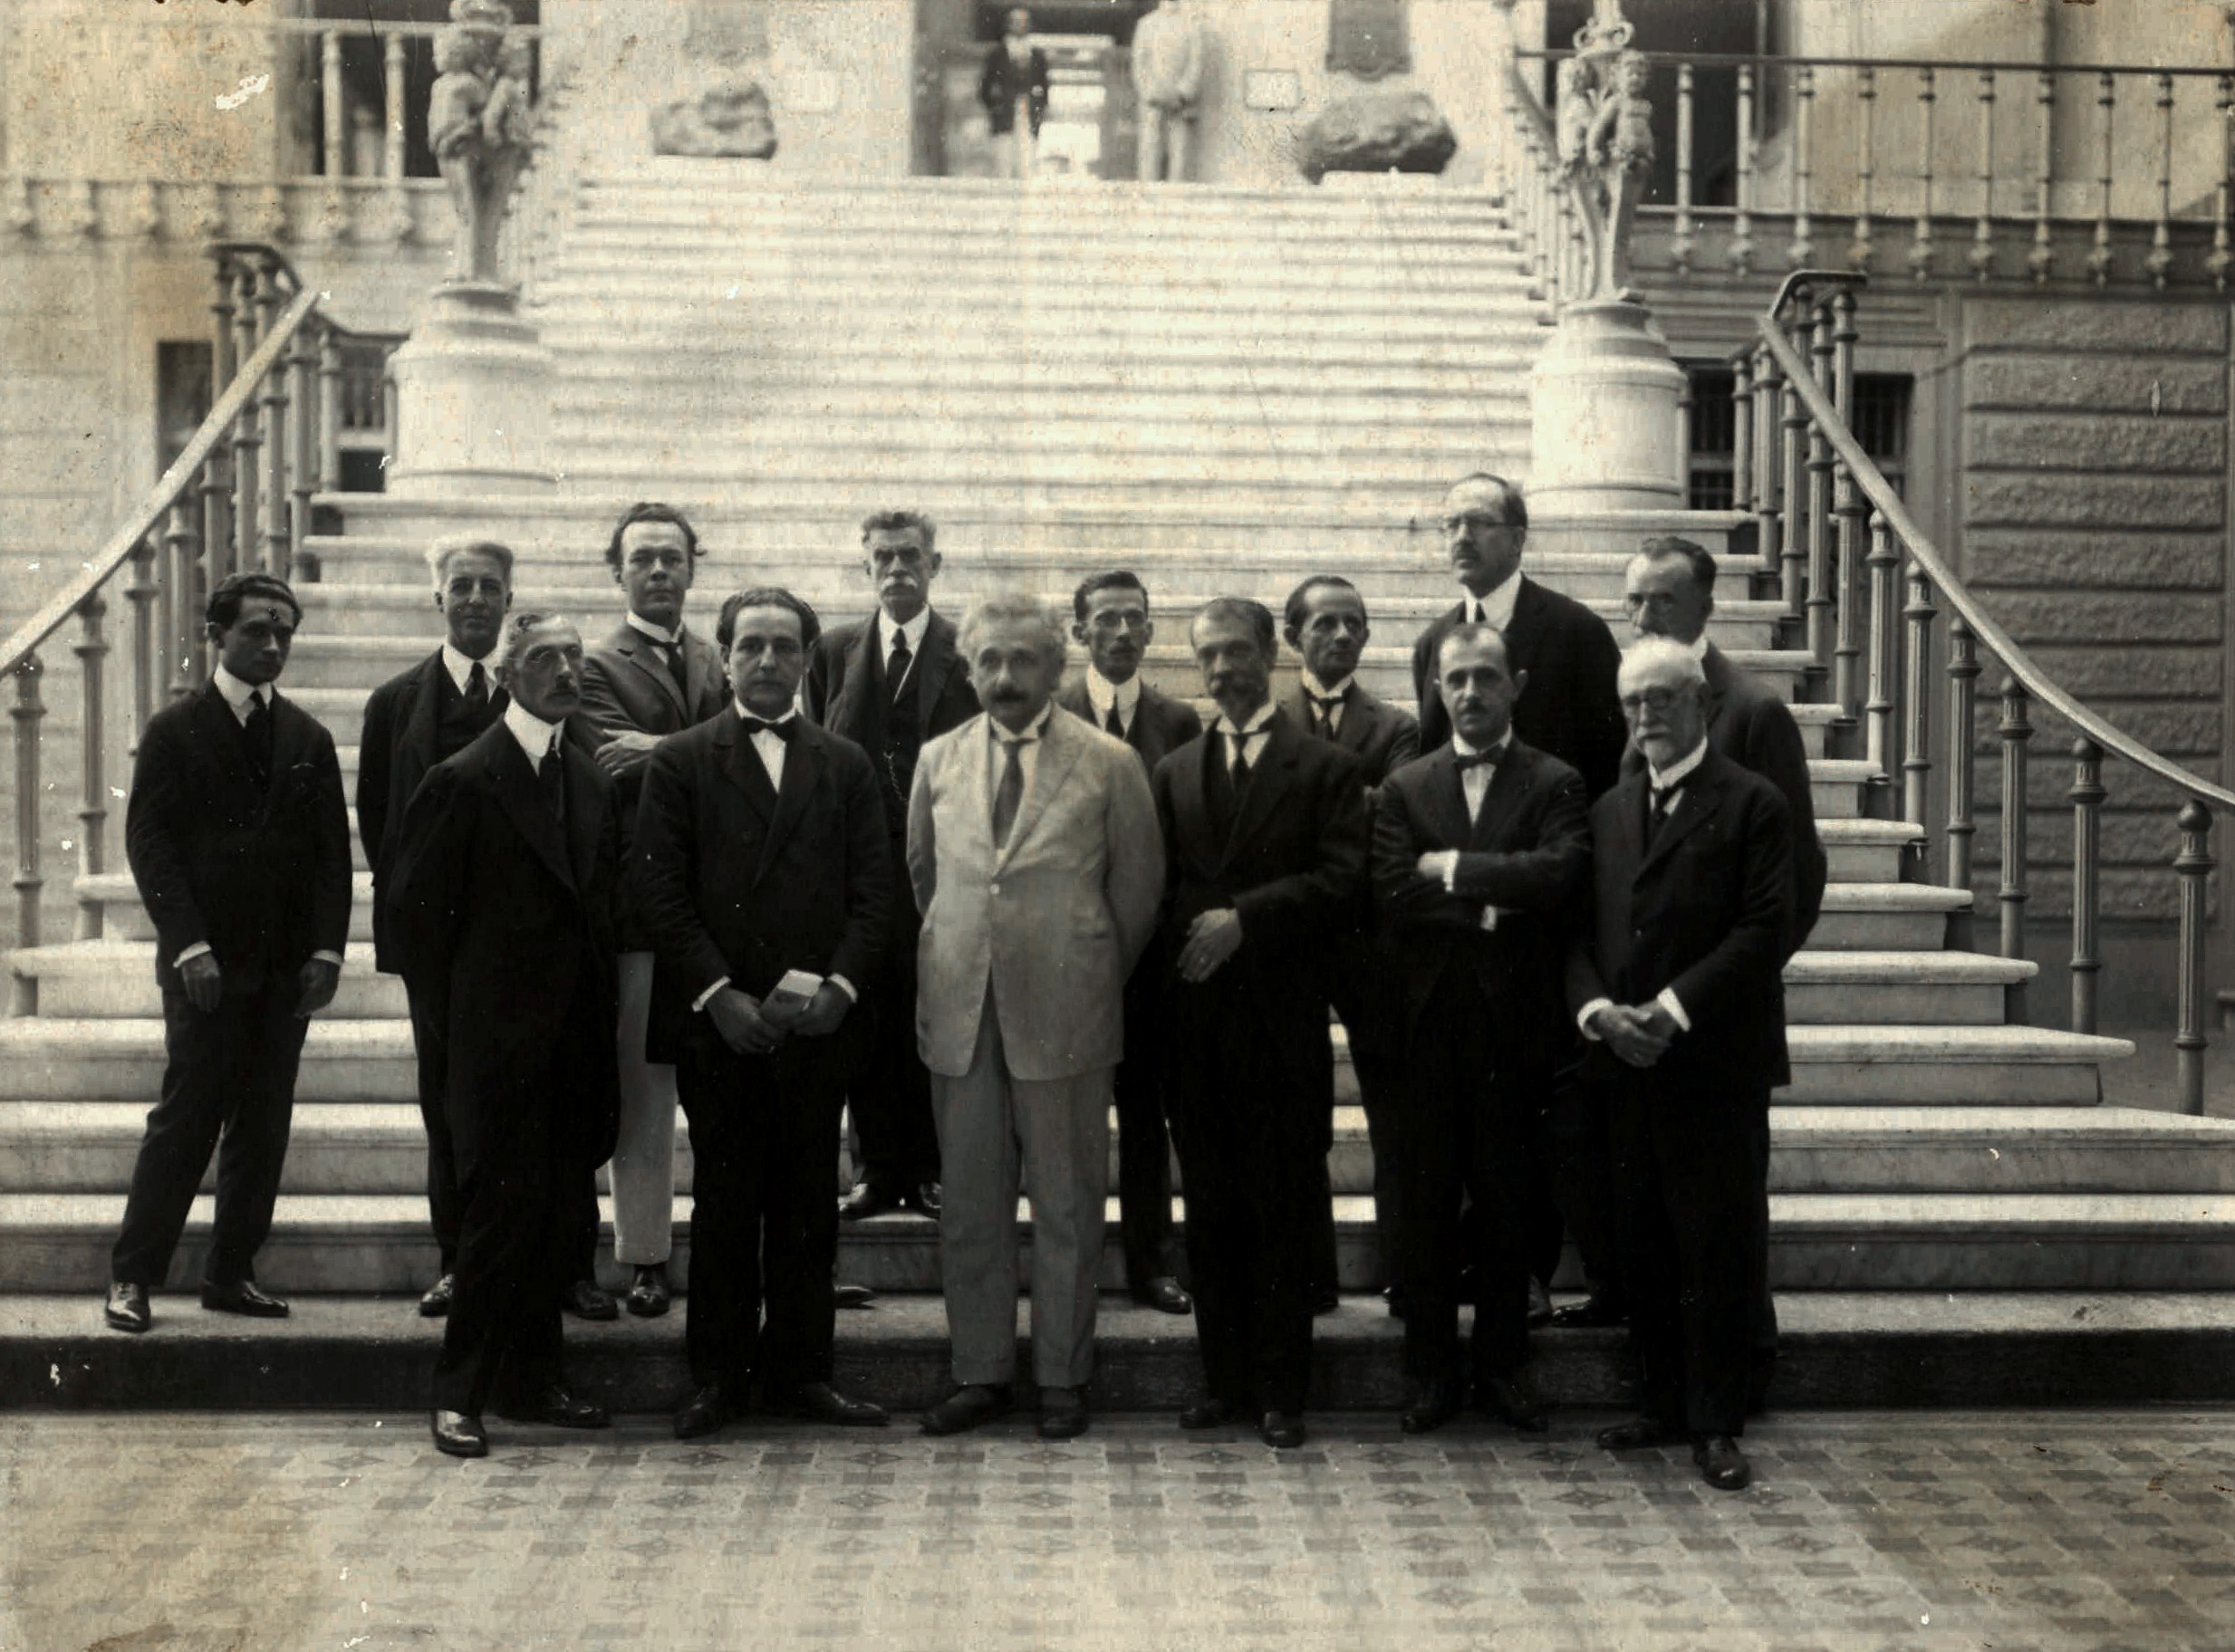
\includegraphics[height=4.85cm]{assets/einstein_museu_nacional_1925.jpg}};
    \end{tikzpicture}

    \vspace{0.1cm}
    \imgcredit{Einstein no Museu Nacional, Rio de Janeiro, 07/05/1925, domínio público}

    \column{0.44\textwidth}
    A visita de Einstein ao Brasil faz parte da circulação internacional da relatividade.

    \vspace{0.25cm}
    \begin{itemize}
      \item Passou pelo Rio de Janeiro em maio de 1925.
      \item Visitou instituições científicas e culturais.
      \item O episódio mostra o Brasil não só como local de observação, mas como parte da recepção pública da nova física.
    \end{itemize}
  \end{columns}
\end{frame}

\begin{frame}{Por que Sobral importa nesta apresentação?}
  Mercúrio e Sobral testam a mesma teoria por caminhos diferentes.

  \vspace{0.3cm}
  \begin{table}
    \centering
    \begin{tabular}{lll}
      \toprule
      Teste & Observável & Previsão relativística \\
      \midrule
      Mercúrio & avanço do periélio & $43\arcsec/\text{século}$ \\
      Sobral/Príncipe & desvio da luz solar & $1{,}75\arcsec$ \\
      \bottomrule
    \end{tabular}
  \end{table}

  \vspace{0.35cm}
  O primeiro explicou uma anomalia antiga; o segundo tornou a teoria mundialmente conhecida.
\end{frame}

\section{Crash course em relatividade geral}

\begin{frame}{Ideia 1: queda livre apaga a gravidade local}
  O ponto de partida físico é o princípio da equivalência:

  \vspace{0.25cm}
  \[
    \text{massa gravitacional} = \text{massa inercial}.
  \]

  \vspace{0.25cm}
  Em uma pequena região em queda livre, os efeitos da gravidade desaparecem localmente. O que resta não é uma força comum, mas a geometria do espaço-tempo.

  \vspace{0.35cm}
  \begin{columns}[T,onlytextwidth]
    \column{0.48\textwidth}
    \centering
    {\color{MercuryMuted}Newton}
    \[
      m\vec a = -\frac{GMm}{r^2}\hat r
    \]
    A gravidade acelera corpos.

    \column{0.48\textwidth}
    \centering
    {\color{MercuryMuted}Einstein}
    \[
      \text{corpos livres seguem geodésicas}
    \]
    A gravidade curva trajetórias.
  \end{columns}
\end{frame}

\begin{frame}{Ideia 2: a métrica mede distâncias no espaço-tempo}
  Em relatividade geral, o objeto central é a métrica $g_{\mu\nu}$:
  \[
    ds^2 = g_{\mu\nu}\,dx^\mu dx^\nu.
  \]

  \vspace{0.25cm}
  Ela diz como medir intervalos, tempos próprios, comprimentos e cones de luz.

  \vspace{0.35cm}
  No espaço-tempo plano da relatividade especial:
  \[
    ds^2 = -c^2dt^2 + dx^2 + dy^2 + dz^2.
  \]

  \vspace{0.25cm}
  Perto de uma massa, a métrica deixa de ser plana. Essa diferença é o campo gravitacional em linguagem geométrica.
\end{frame}

\begin{frame}{Ideia 3: partículas livres seguem geodésicas}
  Uma geodésica é a trajetória ``mais reta possível'' em um espaço-tempo curvo.

  \vspace{0.25cm}
  Sua equação é:
  \[
    \frac{d^2x^\mu}{d\tau^2}
    +
    \Gamma^\mu_{\alpha\beta}
    \frac{dx^\alpha}{d\tau}
    \frac{dx^\beta}{d\tau}
    = 0.
  \]

  \vspace{0.25cm}
  Os símbolos $\Gamma^\mu_{\alpha\beta}$ são calculados a partir da métrica e codificam como o espaço-tempo muda de ponto a ponto.

  \vspace{0.35cm}
  Para Mercúrio, a órbita é uma geodésica na geometria produzida pelo Sol. A precessão aparece porque essa geometria não é exatamente newtoniana.
\end{frame}

\begin{frame}{Geodésica: reta local, curva global}
  Uma geodésica não precisa parecer reta quando vista de fora.

  \vspace{0.25cm}
  O ponto é local: quem caminha sobre a superfície segue sempre ``em frente'', sem virar para a esquerda ou para a direita.

  \vspace{0.25cm}
  \begin{columns}[T,onlytextwidth]
    \column{0.48\textwidth}
    \centering
    {\color{MercuryAccent}\textbf{Plano}}
    \vspace{0.1cm}

    \begin{tikzpicture}[scale=0.85]
      \draw[MercuryLine] (-2,-1.35) grid[step=0.45] (2,1.35);
      \draw[MercuryOrbit,line width=1.1pt,->] (-1.6,-0.65) -- (1.6,0.65);
      \fill[MercuryAccent] (-1.6,-0.65) circle (0.05);
      \fill[MercuryAccent] (1.6,0.65) circle (0.05);
      \node[text=MercuryMuted,scale=0.75] at (0,-1.75) {geodésica = reta usual};
    \end{tikzpicture}

    \column{0.48\textwidth}
    \centering
    {\color{MercuryAccent}\textbf{Esfera}}
    \vspace{0.1cm}

    \begin{tikzpicture}[scale=0.85]
      \shade[ball color=MercuryLine!55!MercuryBlack,opacity=0.9] (0,0) circle (1.35);
      \draw[MercuryMuted,opacity=0.45] (0,0) ellipse (1.35 and 0.35);
      \draw[MercuryOrbit,line width=1.1pt,->] (0,-1.35) arc[start angle=-90,end angle=110,radius=1.35];
      \fill[MercuryAccent] (0,-1.35) circle (0.05);
      \fill[MercuryAccent] (-0.46,1.27) circle (0.05);
      \node[text=MercuryMuted,scale=0.75] at (0,-1.75) {geodésica = grande círculo};
    \end{tikzpicture}
  \end{columns}

  \vspace{0.25cm}
  A palavra ``reta'' passa a significar: trajetória que não tem aceleração própria.
\end{frame}

\begin{frame}{A analogia das formigas na esfera}
  Imagine formigas vivendo sobre uma esfera enorme.

  \vspace{0.25cm}
  Para cada formiga, uma pequena vizinhança parece plana: ela pode desenhar régua, ângulo reto e linhas locais sem perceber a curvatura.

  \vspace{0.25cm}
  Mas elas podem descobrir a curvatura sem sair da superfície:
  \begin{itemize}
    \item caminham sempre em frente, seguindo geodésicas;
    \item comparam trajetórias inicialmente paralelas;
    \item observam que essas trajetórias se aproximam e podem se cruzar.
  \end{itemize}

  \vspace{0.25cm}
  Essa é a moral da explicação popularizada por Kip Thorne: curvatura não precisa ser vista de fora; ela pode ser medida por experiências internas.
\end{frame}

\begin{frame}{Formigas: paralelas que se encontram}
  \begin{columns}[T,onlytextwidth]
    \column{0.48\textwidth}
    \centering
    {\color{MercuryAccent}\textbf{No plano}}

    \vspace{0.15cm}
    \begin{tikzpicture}[scale=0.9]
      \draw[MercuryLine] (-2.2,-1.5) grid[step=0.5] (2.2,1.5);
      \draw[MercuryOrbit,line width=1.2pt,->] (-1.75,-1.0) -- (1.75,-1.0);
      \draw[MercuryOrbit,line width=1.2pt,->] (-1.75,0.45) -- (1.75,0.45);
      \fill[MercuryAccent] (-1.75,-1.0) circle (0.06);
      \fill[MercuryAccent] (-1.75,0.45) circle (0.06);
      \node[text=MercuryMuted,scale=0.72,align=center] at (0,-1.85)
        {linhas paralelas\\mantêm distância};
    \end{tikzpicture}

    \column{0.48\textwidth}
    \centering
    {\color{MercuryAccent}\textbf{Na esfera}}

    \vspace{0.15cm}
    \begin{tikzpicture}[scale=0.9]
      \shade[ball color=MercuryLine!55!MercuryBlack,opacity=0.92] (0,0) circle (1.55);
      \draw[MercuryMuted,opacity=0.42] (0,0) ellipse (1.55 and 0.42);
      \draw[MercuryMuted,opacity=0.28] (0,0) ellipse (0.72 and 1.55);
      \draw[MercuryOrbit,line width=1.15pt,->] (-0.75,-1.35) .. controls (-1.15,-0.45) and (-0.78,0.55) .. (0,1.55);
      \draw[MercuryRelativity,line width=1.15pt,->] (0.75,-1.35) .. controls (1.15,-0.45) and (0.78,0.55) .. (0,1.55);
      \fill[MercuryAccent] (-0.75,-1.35) circle (0.055);
      \fill[MercuryAccent] (0.75,-1.35) circle (0.055);
      \fill[MercuryText] (0,1.55) circle (0.045);
      \node[text=MercuryMuted,scale=0.72,align=center] at (0,-1.95)
        {meridianos começam paralelos\\e se cruzam no polo};
    \end{tikzpicture}
  \end{columns}

  \vspace{0.2cm}
  Em uma geometria curva, a separação entre geodésicas revela a curvatura.
\end{frame}

\begin{frame}{Curvatura medida por triângulos}
  Outra experiência interna: desenhar um triângulo com geodésicas.

  \vspace{0.2cm}
  \begin{columns}[T,onlytextwidth]
    \column{0.48\textwidth}
    \centering
    {\color{MercuryAccent}\textbf{Plano euclidiano}}

    \vspace{0.2cm}
    \begin{tikzpicture}[scale=0.92]
      \draw[MercuryOrbit,line width=1.1pt] (-1.55,-1.05) -- (1.35,-1.05) -- (-0.5,1.15) -- cycle;
      \node[text=MercuryText] at (-0.82,-0.75) {$\alpha$};
      \node[text=MercuryText] at (0.88,-0.75) {$\beta$};
      \node[text=MercuryText] at (-0.32,0.73) {$\gamma$};
      \node[text=MercuryMuted,scale=0.78] at (0,-1.65) {$\alpha+\beta+\gamma=180^\circ$};
    \end{tikzpicture}

    \column{0.48\textwidth}
    \centering
    {\color{MercuryAccent}\textbf{Esfera}}

    \vspace{0.2cm}
    \begin{tikzpicture}[scale=0.92]
      \shade[ball color=MercuryLine!55!MercuryBlack,opacity=0.9] (0,0) circle (1.45);
      \draw[MercuryMuted,opacity=0.42] (0,0) ellipse (1.45 and 0.36);
      \draw[MercuryOrbit,line width=1.1pt] (-1.2,0) arc[start angle=180,end angle=360,x radius=1.2,y radius=0.3];
      \draw[MercuryOrbit,line width=1.1pt] (-1.2,0) .. controls (-0.72,0.85) and (-0.35,1.25) .. (0,1.45);
      \draw[MercuryOrbit,line width=1.1pt] (1.2,0) .. controls (0.72,0.85) and (0.35,1.25) .. (0,1.45);
      \node[text=MercuryText,scale=0.8] at (-0.78,0.12) {$90^\circ$};
      \node[text=MercuryText,scale=0.8] at (0.78,0.12) {$90^\circ$};
      \node[text=MercuryText,scale=0.8] at (0,1.05) {$90^\circ$};
      \node[text=MercuryMuted,scale=0.78] at (0,-1.75) {$90^\circ+90^\circ+90^\circ>180^\circ$};
    \end{tikzpicture}
  \end{columns}

  \vspace{0.25cm}
  A soma dos ângulos de um triângulo é uma medida de curvatura.
\end{frame}

\begin{frame}{Da esfera ao espaço-tempo}
  A analogia da esfera tem uma limitação: ela é uma superfície curva embutida em um espaço externo.

  \vspace{0.25cm}
  Na relatividade geral, não precisamos imaginar um ``lado de fora'' do espaço-tempo.

  \vspace{0.25cm}
  A curvatura aparece em experiências internas:
  \begin{itemize}
    \item geodésicas que convergem ou divergem;
    \item relógios que acumulam tempos próprios diferentes;
    \item luz que muda de direção perto do Sol;
    \item órbitas que não fecham exatamente.
  \end{itemize}

  \vspace{0.3cm}
  Mercúrio é uma dessas experiências internas: ele segue sempre uma geodésica, mas a geometria solar faz o periélio avançar.
\end{frame}

\begin{frame}{Não precisamos de um lado de fora}
  A curvatura pode ser descrita apenas por medidas feitas dentro do próprio espaço.

  \vspace{0.2cm}
  \begin{columns}[T,onlytextwidth]
    \column{0.48\textwidth}
    \centering
    {\color{MercuryAccent}\textbf{Imagem intuitiva}}

    \vspace{0.15cm}
    \begin{tikzpicture}[scale=0.86]
      \shade[ball color=MercuryLine!55!MercuryBlack,opacity=0.9] (0,0) circle (1.45);
      \draw[MercuryOrbit,line width=1pt] (-1.15,-0.05) arc[start angle=190,end angle=350,x radius=1.17,y radius=0.31];
      \draw[MercuryRelativity,line width=1pt] (-0.1,-1.43) arc[start angle=-94,end angle=96,radius=1.43];
      \node[text=MercuryMuted,scale=0.75,align=center] at (0,-1.95) {a esfera parece curva\\vista de fora};
    \end{tikzpicture}

    \column{0.48\textwidth}
    \centering
    {\color{MercuryAccent}\textbf{Descrição física}}

    \vspace{0.15cm}
    \begin{tikzpicture}[scale=0.86]
      \draw[MercuryLine] (-2,-1.35) rectangle (2,1.35);
      \draw[MercuryOrbit,line width=1pt] (-1.55,-0.75) .. controls (-0.5,-0.2) and (0.55,0.2) .. (1.55,0.75);
      \draw[MercuryRelativity,line width=1pt] (-1.5,0.75) .. controls (-0.45,0.1) and (0.45,-0.1) .. (1.5,-0.75);
      \node[fill=MercuryBlack,inner xsep=4pt,inner ysep=2pt,text=MercuryText,scale=0.82]
        at (0,-1.02) {$ds^2=g_{\mu\nu}dx^\mu dx^\nu$};
      \node[text=MercuryMuted,scale=0.75,align=center] at (0,-1.9) {a métrica contém\\toda a geometria};
    \end{tikzpicture}
  \end{columns}

  \vspace{0.25cm}
  Na relatividade geral, a pergunta operacional é: que medidas relógios, réguas, luz e partículas livres fazem?
\end{frame}

\begin{frame}{Experiência interna 1: geodésicas convergem}
  Se duas partículas livres partem próximas, a curvatura pode mudar a separação entre elas.

  \vspace{0.2cm}
  \begin{columns}[T,onlytextwidth]
    \column{0.5\textwidth}
    \centering
    \begin{tikzpicture}[scale=0.92]
      \draw[MercuryLine] (-2.2,-1.4) grid[step=0.45] (2.2,1.4);
      \draw[MercuryOrbit,line width=1.1pt,->] (-1.9,-0.65) .. controls (-0.6,-0.45) and (0.65,-0.35) .. (1.9,-0.2);
      \draw[MercuryRelativity,line width=1.1pt,->] (-1.9,0.65) .. controls (-0.6,0.45) and (0.65,0.35) .. (1.9,0.2);
      \draw[MercuryAccent,<->] (-1.75,-0.62) -- (-1.75,0.62);
      \draw[MercuryAccent,<->] (1.65,-0.22) -- (1.65,0.22);
      \node[text=MercuryMuted,scale=0.75] at (0,-1.85) {a separação muda mesmo sem forças locais};
    \end{tikzpicture}

    \column{0.46\textwidth}
    A equação de desvio geodésico resume a ideia:
    \[
      \frac{D^2\xi^\mu}{d\tau^2}
      =
      -R^\mu{}_{\nu\alpha\beta}
      u^\nu\xi^\alpha u^\beta.
    \]

    \vspace{0.2cm}
    Aqui $\xi^\mu$ é a separação entre trajetórias vizinhas.

    \vspace{0.2cm}
    Se $R^\mu{}_{\nu\alpha\beta}\neq 0$, a curvatura tem efeitos mensuráveis.
  \end{columns}
\end{frame}

\begin{frame}{Experiência interna 2: relógios e tempo próprio}
  Relógios em regiões gravitacionais diferentes não precisam marcar o mesmo tempo próprio.

  \vspace{0.12cm}
  \begin{columns}[T,onlytextwidth]
    \column{0.5\textwidth}
    \centering
    \begin{tikzpicture}[scale=0.88]
      \fill[MercuryAccent] (0,0) circle (0.32);
      \foreach \r in {0.85,1.45,2.05} {
        \draw[MercuryLine] (0,0) circle (\r);
      }
      \draw[MercuryOrbit,->,line width=1pt] (1.45,0) arc[start angle=0,end angle=70,radius=1.45];
      \draw[MercuryRelativity,->,line width=1pt] (2.05,0) arc[start angle=0,end angle=70,radius=2.05];
      \node[draw=MercuryLine,circle,text=MercuryText,minimum size=0.34cm] at (1.45,0) {};
      \node[draw=MercuryLine,circle,text=MercuryText,minimum size=0.34cm] at (2.05,0) {};
      \node[text=MercuryMuted,scale=0.7] at (1.28,-0.35) {$r_1$};
      \node[text=MercuryMuted,scale=0.7] at (2.18,-0.35) {$r_2$};
      \node[text=MercuryMuted,scale=0.75,align=center] at (0,-2.25) {relógios medem\\tempo próprio};
    \end{tikzpicture}

    \column{0.46\textwidth}
    No campo de Schwarzschild, para um relógio parado a raio $r$:
    \[
      d\tau =
      \sqrt{1-\frac{2GM}{rc^2}}\,dt.
    \]

    \vspace{0.04cm}
    Mais perto da massa:
    \[
      d\tau < dt.
    \]

    \vspace{0.02cm}
    Curvatura também é testada por relógios.

    \vspace{0.06cm}
    {\color{MercuryAccent}\scriptsize
    \href{dashboard_tempo_proprio.html}{Abrir dashboard interativo: variar $r$ e $t$}}

    \vspace{0.02cm}
    {\tiny\color{MercuryMuted}
    fallback: abrir \texttt{dashboard\_tempo\_proprio.html} na pasta da apresentação}
  \end{columns}
\end{frame}

\begin{frame}{Experiência interna 3: luz muda de direção}
  \begin{columns}[T,onlytextwidth]
    \column{0.42\textwidth}
    \centering
    \begin{tikzpicture}
      \node[
        draw=MercuryLine,
        line width=0.45pt,
        inner sep=2pt
      ]{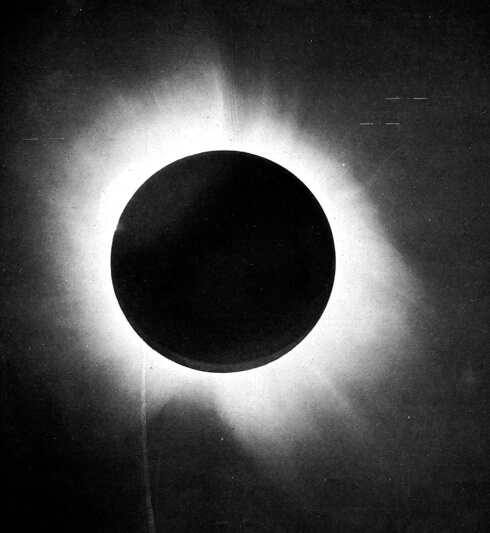
\includegraphics[height=4.05cm]{assets/sobral_1919_eclipse_positive.jpg}};
    \end{tikzpicture}

    \vspace{0.1cm}
    \imgcredit{Eclipse de Sobral, 1919, domínio público}

    \column{0.54\textwidth}
    A luz não tem massa de repouso, mas segue geodésicas nulas: $ds^2=0$.

    \vspace{0.15cm}
    Perto do Sol, essas geodésicas são desviadas:
    \[
      \alpha \approx \frac{4GM_\odot}{c^2 b}.
    \]

    \vspace{0.15cm}
    Para um raio passando próximo à borda solar:
    \[
      \alpha \approx 1{,}75\arcsec.
    \]

    \vspace{0.1cm}
    Sobral testou exatamente esse tipo de experiência interna: observar posições aparentes de estrelas.
  \end{columns}
\end{frame}

\begin{frame}{Experiência interna 4: órbitas não fecham}
  \begin{columns}[T,onlytextwidth]
    \column{0.42\textwidth}
    \centering
    \begin{tikzpicture}
      \node[
        draw=MercuryLine,
        line width=0.45pt,
        inner sep=2pt
      ]{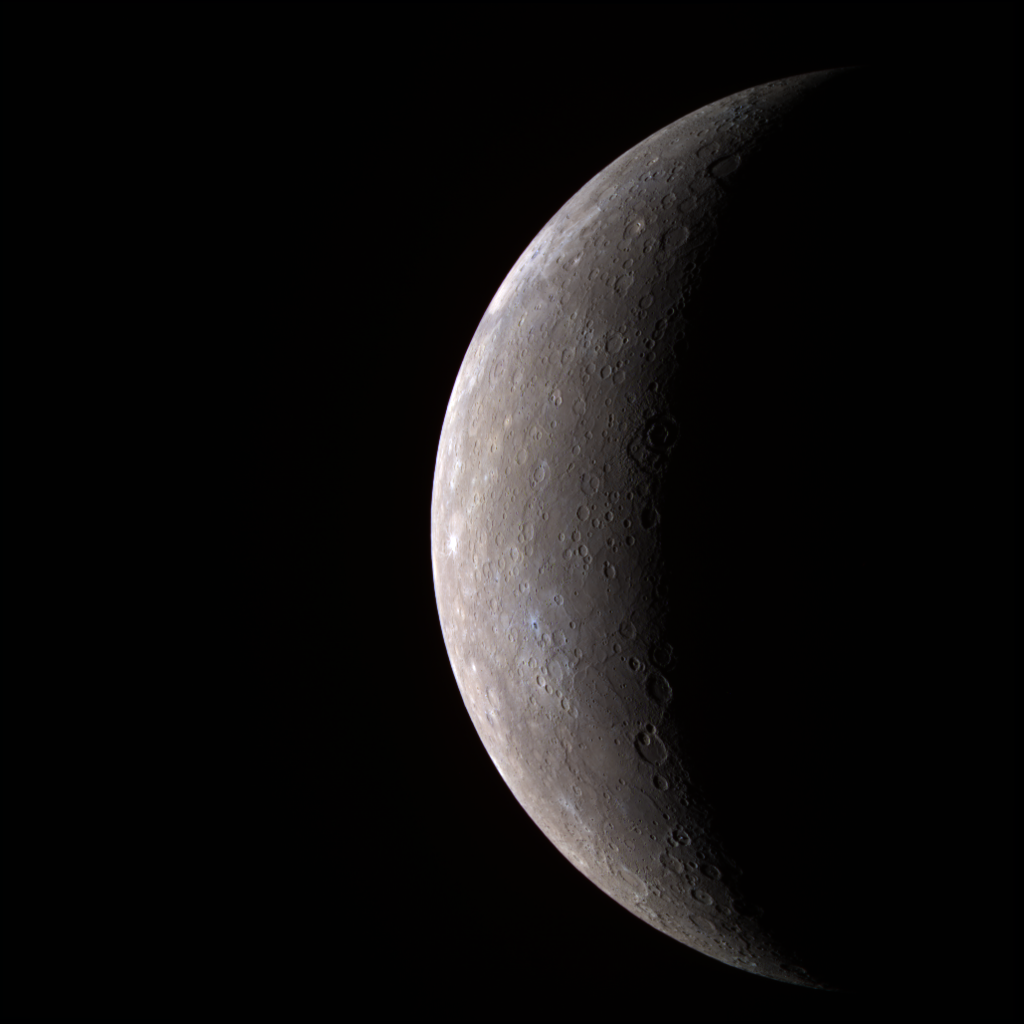
\includegraphics[height=4.3cm]{assets/mercury_messenger.png}};
    \end{tikzpicture}

    \vspace{0.1cm}
    \imgcredit{Mercúrio, NASA/MESSENGER}

    \column{0.54\textwidth}
    A órbita de Mercúrio é uma geodésica na geometria do Sol.

    \vspace{0.2cm}
    No limite newtoniano ideal, a elipse fecha.

    \vspace{0.2cm}
    Na geometria relativística, surge um avanço:
    \[
      \Delta\varpi =
      \frac{6\pi GM_\odot}{a(1-e^2)c^2}.
    \]

    \vspace{0.2cm}
    A cada volta, o periélio retorna ligeiramente deslocado.
  \end{columns}
\end{frame}

\begin{frame}{O mesmo diagnóstico em quatro observáveis}
  \begin{table}
    \centering
    \begin{tabular}{lll}
      \toprule
      Observável & O que se mede & Sinal de curvatura \\
      \midrule
      Geodésicas próximas & separação $\xi^\mu$ & convergência/divergência \\
      Relógios & tempo próprio $\tau$ & ritmos diferentes \\
      Luz & posição aparente de estrelas & deflexão angular \\
      Órbitas & retorno ao periélio & elipse não fecha \\
      \bottomrule
    \end{tabular}
  \end{table}

  \vspace{0.35cm}
  A relatividade geral não pede para visualizar uma quarta dimensão espacial.
  Ela pede para medir como trajetórias, luz e relógios se comportam.

  \vspace{0.25cm}
  Mercúrio é o caso orbital dessa lista; Sobral é o caso óptico.
\end{frame}

\begin{frame}{Ideia 4: matéria diz ao espaço-tempo como curvar}
  As equações de Einstein conectam geometria e conteúdo físico:
  \[
    G_{\mu\nu}
    =
    \frac{8\pi G}{c^4}T_{\mu\nu}.
  \]

  \vspace{0.25cm}
  \begin{columns}[T,onlytextwidth]
    \column{0.48\textwidth}
    \centering
    {\color{MercuryMuted}Geometria}
    \[
      G_{\mu\nu}
    \]
    Curvatura do espaço-tempo.

    \column{0.48\textwidth}
    \centering
    {\color{MercuryMuted}Matéria e energia}
    \[
      T_{\mu\nu}
    \]
    Massa, energia, pressão e fluxos.
  \end{columns}

  \vspace{0.35cm}
  Fora de uma estrela esférica e não rotante, a solução é a métrica de Schwarzschild, usada para calcular a precessão relativística de Mercúrio.
\end{frame}

\begin{frame}{Ideia 5: Newton reaparece como aproximação}
  A relatividade geral precisa recuperar Newton quando o campo é fraco e as velocidades são pequenas:
  \[
    v \ll c,
    \qquad
    \frac{GM}{rc^2}\ll 1.
  \]

  \vspace{0.3cm}
  Nesse limite, a componente temporal da métrica contém o potencial newtoniano:
  \[
    g_{00} \approx -\left(1+\frac{2\Phi}{c^2}\right),
    \qquad
    \Phi = -\frac{GM}{r}.
  \]

  \vspace{0.3cm}
  Mercúrio vive quase nesse regime. O ``quase'' é precisamente o suficiente para produzir os $43\arcsec$ por século.
\end{frame}

\section{Atividades e fechamento}

\begin{frame}{Atividade 1: lendo o dashboard}
  Abra o dashboard e teste três cenários:

  \vspace{0.25cm}
  \begin{enumerate}
    \item Mercúrio real: $a=0{,}387$ UA, $e=0{,}206$.
    \item Um planeta mais distante: $a=1$ UA, $e=0{,}0167$.
    \item Um planeta próximo e excêntrico: $a=0{,}25$ UA, $e=0{,}6$.
  \end{enumerate}

  \vspace{0.35cm}
  Pergunta para discussão:
  \[
    \text{qual parâmetro muda mais dramaticamente a precessão: }a\text{ ou }e?
  \]
\end{frame}

\begin{frame}{Atividade 2: estimativa de ordem de grandeza}
  Use
  \[
    \Delta\varpi =
    \frac{6\pi GM}{a(1-e^2)c^2}
  \]
  para comparar Mercúrio e Terra.

  \vspace{0.3cm}
  \begin{columns}[T,onlytextwidth]
    \column{0.48\textwidth}
    {\color{MercuryAccent}\textbf{Mercúrio}}
    \[
      a=0{,}387\,\text{UA},
      \qquad e=0{,}206
    \]

    \column{0.48\textwidth}
    {\color{MercuryAccent}\textbf{Terra}}
    \[
      a=1\,\text{UA},
      \qquad e=0{,}0167
    \]
  \end{columns}

  \vspace{0.35cm}
  O objetivo não é decorar números: é ver como a estrutura da fórmula decide qual órbita é o melhor teste.
\end{frame}

\begin{frame}{Atividade 3: debate histórico}
  Divida a turma em três grupos:

  \vspace{0.25cm}
  \begin{itemize}
    \item \textbf{Grupo Newtoniano:} defender a busca por Vulcano ou matéria intramercurial.
    \item \textbf{Grupo Relativista:} defender uma mudança conceitual na teoria da gravitação.
    \item \textbf{Grupo Observacional:} exigir critérios de evidência, erro e reprodutibilidade.
  \end{itemize}

  \vspace{0.35cm}
  Pergunta-guia:
  \[
    \text{quando uma anomalia exige remendo, e quando exige nova teoria?}
  \]
\end{frame}

\begin{frame}{Síntese para duas aulas}
  \begin{columns}[T,onlytextwidth]
    \column{0.48\textwidth}
    {\color{MercuryAccent}\textbf{Aula 1}}
    \vspace{0.2cm}
    \begin{itemize}
      \item uma anomalia pequena pode ser profunda;
      \item Newton não ``falhou'' simplesmente: chegou ao limite de validade;
      \item o sucesso de Netuno tornou Vulcano uma hipótese razoável.
    \end{itemize}

    \column{0.48\textwidth}
    {\color{MercuryAccent}\textbf{Aula 2}}
    \vspace{0.2cm}
    \begin{itemize}
      \item a RG explica Mercúrio por geometria;
      \item Sobral testou a curvatura da luz;
      \item Einstein veio ao Brasil em 1925, não na expedição de 1919.
    \end{itemize}
  \end{columns}

  \vspace{0.4cm}
  \centering
  \goldline
\end{frame}

\begin{frame}{Conclusão}
  A precessão de Mercúrio mostra como uma pequena discrepância pode revelar uma mudança profunda de teoria.

  \vspace{0.35cm}
  \begin{itemize}
    \item Newton explicou quase toda a mecânica planetária com enorme precisão.
    \item Mercúrio deixou um resíduo de cerca de $43\arcsec$ por século.
    \item Hipóteses newtonianas auxiliares não se sustentaram.
    \item A relatividade geral explicou o resíduo como efeito da curvatura do espaço-tempo perto do Sol.
  \end{itemize}

  \vspace{0.35cm}
  O problema de Mercúrio tornou-se um dos primeiros grandes testes observacionais da nova teoria da gravitação.
\end{frame}

\begin{frame}{Referências essenciais}
  \begin{thebibliography}{99}
    \bibitem{einstein1915}
    A. Einstein,
    \textit{Explanation of the Perihelion Motion of Mercury from the General Theory of Relativity},
    1915.

    \bibitem{weinberg}
    S. Weinberg,
    \textit{Gravitation and Cosmology},
    Wiley, 1972.

    \bibitem{carroll}
    S. Carroll,
    \textit{Spacetime and Geometry},
    Addison-Wesley, 2004.

    \bibitem{will}
    C. M. Will,
    \textit{Theory and Experiment in Gravitational Physics},
    Cambridge University Press, 1993.

    \bibitem{dyson1920}
    F. W. Dyson, A. S. Eddington e C. Davidson,
    \textit{A Determination of the Deflection of Light by the Sun's Gravitational Field},
    1920.

    \bibitem{nature1919}
    \textit{Nature},
    \textit{Results of the Total Solar Eclipse of May 29 and the Relativity Theory},
    1919.
  \end{thebibliography}
\end{frame}

\begin{frame}{Fontes visuais e históricas}
  \begin{thebibliography}{99}
    \bibitem{eclipse1919}
    Eclipse 1919,
    \textit{The Sobral expedition}.

    \bibitem{cbpf}
    Centro Brasileiro de Pesquisas Físicas,
    \textit{O eclipse de Sobral: o Brasil no mapa da teoria da relatividade}.

    \bibitem{abc}
    Academia Brasileira de Ciências,
    \textit{Einstein at the Brazilian Academy of Sciences}.

    \bibitem{commons}
    Wikimedia Commons:
    imagens de Mercúrio/MESSENGER, Newton, Le Verrier, Eddington,
    eclipse de Sobral e Einstein no Museu Nacional.
  \end{thebibliography}
\end{frame}

\end{document}
